\documentclass[11pt,a4paper]{article}

% ---------------------------------------------------------------------------
% Reporte técnico — GeoStats
% Compilar:  cd docs/reporte && latexmk -pdf reporte.tex
% Las figuras vienen de los notebooks (notebooks/*.qmd); se extraen del HTML
% renderizado y viven en figuras/. No se editan a mano.
% ---------------------------------------------------------------------------

\usepackage[utf8]{inputenc}
\usepackage[T1]{fontenc}
\usepackage[spanish,es-tabla,es-noquoting]{babel}
\usepackage{lmodern}
\usepackage{microtype}
\usepackage{geometry}
\geometry{margin=2.6cm}
\usepackage{amsmath,amssymb}
\usepackage{booktabs}
\usepackage{graphicx}
\graphicspath{{figuras/}}
\usepackage{float}
\usepackage{caption}
\captionsetup{font=small,labelfont=bf,width=0.92\textwidth}
\usepackage{xcolor}
\definecolor{azul}{HTML}{005991}
\definecolor{rojo}{HTML}{8B2C1A}
\definecolor{grafito}{HTML}{2C2C2C}
\usepackage[colorlinks=true,linkcolor=azul,citecolor=azul,urlcolor=azul]{hyperref}
\usepackage{enumitem}
\setlist{nosep}
\usepackage{multirow}
\usepackage{array}
\usepackage{tcolorbox}
\tcbuselibrary{skins,breakable}
\newtcolorbox{decision}[1]{colback=white,colframe=rojo,fonttitle=\bfseries,
  title={Decisión: #1},breakable,left=4pt,right=4pt,top=3pt,bottom=3pt}
\newtcolorbox{advertencia}{colback=gray!6,colframe=grafito,breakable,
  left=4pt,right=4pt,top=3pt,bottom=3pt}

\newcommand{\NB}{\mathrm{BinomialNegativa}}
\newcommand{\Pois}{\mathrm{Poisson}}
\newcommand{\E}{\mathbb{E}}
\newcommand{\Var}{\mathrm{Var}}
\newcommand{\Rhat}{\hat{R}}

\title{\textbf{Predicción espacial de accidentes de tránsito\\en la Zona Metropolitana de Monterrey}\\[6pt]
\large Procedimientos, razonamiento y resultados del proyecto GeoStats}
\author{Eduardo Luna\\\small Tecnológico de Monterrey}
\date{Septiembre de 2026}

\begin{document}
\maketitle

\begin{abstract}
\noindent
Este reporte documenta el recorrido metodológico completo del proyecto: desde
la pregunta original —predecir cuántos accidentes de tránsito ocurrirán y en
qué lugares de la Zona Metropolitana de Monterrey (ZMM)— hasta un modelo
bayesiano jerárquico validado fuera de muestra. Está escrito para que el equipo
entienda no solo \emph{qué} se hizo, sino \emph{por qué} se tomó cada decisión
y qué evidencia la sostiene. Los hallazgos principales son tres. Primero, la
siniestralidad de la ZMM tiene estructura espacial fuerte y persistente: el
5\,\% del territorio con red vial concentra el 44\,\% de los accidentes, la
autocorrelación espacial es alta ($I$ de Moran $= 0{,}65$) y el ranking de
zonas de 2019 correlaciona $0{,}83$ con el de 2024. Segundo, la fuente
dominante del error de predicción no es estadística sino administrativa: los
municipios cambian de \emph{régimen de reporte} de un año a otro, y ningún
modelo puede anticipar eso desde el pasado. Tercero, el modelo jerárquico
final (Binomial Negativa con efecto municipal dinámico y efecto espacial CAR
por celda) supera al mejor \emph{baseline} en calidad distribucional
(CRPS $6{,}17$ contra $6{,}56$) y produce el primer mapa de riesgo relativo neto
del régimen municipal, pero no mueve el índice de precisión predictiva (PAI
$8{,}4$), que está determinado por el historial. Se documentan también los
caminos que no funcionaron y por qué.
\end{abstract}

\tableofcontents
\clearpage

% ===========================================================================
\section{La pregunta y cómo se reformuló}
% ===========================================================================

La pregunta original del equipo era: \emph{¿cuántos accidentes viales habrá, y
en qué AGEBs?} La propuesta inicial contemplaba un proceso de Poisson para el
total, una distribución de probabilidad sobre AGEBs para el reparto, y como
alternativa un clasificador de Bayes. Tres observaciones reorganizaron el
problema antes de tocar un solo dato.

\paragraph{Las dos etapas son un solo modelo.}
Si los conteos por unidad son Poisson independientes, $N_i \sim \Pois(\lambda_i)$,
entonces el total es Poisson con media $\sum_i \lambda_i$ y el reparto
condicional al total es multinomial con probabilidades $\lambda_i/\sum_j \lambda_j$.
Modelar $\lambda_i$ por unidad contesta \emph{cuántos} y \emph{dónde} de una
sola tabla; construir dos modelos y pegarlos obliga a mantener la coherencia a
mano y pierde la propagación de incertidumbre.

\paragraph{Un clasificador contesta otra pregunta.}
Un clasificador estima $P(\text{lugar} \mid \text{accidente})$: dado que ocurrió
un accidente, dónde fue. Nunca dice cuántos habrá. Además, Naive Bayes supone
independencia condicional entre predictores, que aquí es falsa de forma
evidente (hora, día, tipo de vehículo y lugar están enlazados). Se descartó.

\paragraph{Lo que se predice es una intensidad, no un evento.}
A escala fina un accidente individual es casi aleatorio. Lo que se puede
estimar es la \emph{tasa esperada} de cada unidad —qué tan cargada está la
moneda de cada lugar—, no el lanzamiento. Con esa tasa se construyen el
ranking, el total y el mapa. Fijar esa expectativa desde el inicio evita
prometer lo que ningún modelo entrega.

\begin{decision}{marco de modelado}
Panel de conteos por unidad espacial y periodo; modelo lineal generalizado de
conteos con estructura jerárquica; validación temporal fuera de muestra.
\end{decision}

% ===========================================================================
\section{Los datos}
% ===========================================================================

\subsection{Fuente y recorte}

La base es \emph{Accidentes de Tránsito Terrestre en Zonas Urbanas y
Suburbanas} (ATUS) del INEGI, en su versión georreferenciada 2019--2024:
1\,317\,810 registros nacionales con 50 campos. El recorte a la ZMM —los 18
municipios del Sistema Urbano Nacional— deja \textbf{379\,294 registros}, el
100\,\% con coordenadas WGS\,84. El panel de la ZMM está balanceado (los mismos
18 municipios los seis años), lo que no ocurre a nivel nacional (91 municipios
en 2019, 198 en 2024) y es la razón de que las comparaciones temporales se
hagan solo sobre el recorte.

\subsection{Tres propiedades que condicionan todo lo demás}

\begin{enumerate}[leftmargin=1.4em]
\item \textbf{Los faltantes están codificados como valores válidos.} El INEGI
  no usa nulos: ``se ignora'' es un código del catálogo. Solo el 25\,\% de los
  registros tiene información completa en los seis campos con centinelas, y el
  mecanismo es MNAR (en accidentes fatales el aliento alcohólico se ignora
  2,4 veces más seguido). La limpieza \emph{nunca borra filas ni imputa}: solo
  agrega columnas derivadas donde \texttt{isna()} dice la verdad.
\item \textbf{Los registros están referenciados a intersecciones.} El 98,4\,\%
  trae dos vialidades, y el 97,6\,\% de las coordenadas distintas corresponde a
  un único par de calles: ATUS geocodifica la intersección reportada, no el
  punto físico. Lo que existe es un conteo sobre $\sim$60\,000 nodos con
  nombre, no un patrón de puntos continuo. Esto invalida las técnicas planas
  (KDE, $K$ de Ripley) y sugiere que el AGEB descarta resolución que el dato ya
  trae.
\item \textbf{La variable \texttt{URBANA} distingue intersección de tramo.}
  Sus códigos no significan ``urbano/no urbano'' sino ``en intersección'' (96,6\,\%
  en la ZMM) y ``fuera de intersección''. Es la variable que valida el punto
  anterior desde el propio diccionario.
\end{enumerate}

\subsection{Selección de variables}

Las 51 columnas se clasificaron por un criterio que no es estadístico sino
lógico: si la variable describe el \emph{dónde y cuándo} (estructural: existe
haya accidente o no) o el \emph{accidente en sí} (consecuente: solo existe
después del hecho). Las consecuentes —tipo de accidente, vehículos, víctimas,
conductor— \textbf{no pueden ser predictores del conteo}; sirven para
estratificar, para modelos de severidad y para el descriptivo. Quedaron 15
estructurales como predictores potenciales, 18 consecuentes para descriptivo, 5
con reservas y 5 descartadas (\texttt{CINTURON} con 75\,\% de ausencia,
\texttt{MINUTOS} con preferencia de dígito, \texttt{CAPAROD} sin varianza,
\texttt{EDO} constante, y los dos conteos de ``otras víctimas'' casi vacíos).

% ===========================================================================
\section{La unidad espacial}
% ===========================================================================

Se propuso inicialmente el AGEB y se descartó como unidad principal por tres
razones, todas verificables:

\begin{itemize}[leftmargin=1.4em]
\item \textbf{Fronteras sobre avenidas.} Los límites de AGEB se trazan
  frecuentemente sobre vialidades principales, que es justo donde caen los
  accidentes. Un choque en la avenida Constitución cae en la frontera entre
  dos polígonos y su asignación es arbitraria. Es el problema de la unidad de
  área modificable (MAUP) en su forma más dañina para este fenómeno.
\item \textbf{Área heterogénea.} Un AGEB del centro mide 0,2\,km$^2$ y uno
  periférico varios; comparar conteos exige un denominador que casi nunca
  está.
\item \textbf{Vecindad ambigua.} En polígonos irregulares el número de vecinos
  va de 1 a 20, y la matriz de pesos espaciales hereda esa irregularidad.
\end{itemize}

\begin{decision}{rejilla hexagonal de 500\,m de lado}
Hexágonos regulares de 0,65\,km$^2$ (comparables a un AGEB urbano) en
proyección UTM 14N. Área constante (el conteo \emph{es} la densidad), sin sesgo
de frontera (la rejilla no sabe dónde están las calles), seis vecinos
idénticos. Se conservan solo las celdas con al menos un accidente en seis
años —una celda vacía en 379 mil registros no tiene red vial, no es riesgo
cero— y se retiran las 103 celdas isla (sin vecinas con accidentes; 0,07\,\% de
los registros). Quedan \textbf{2\,241 celdas}. El AGEB pasa de ser la unidad a
ser una fuente futura de covariables.
\end{decision}

La partición vive en \texttt{geostats.espacial.celdas()} y es la misma en los
tres notebooks de análisis; cada uno verifica con un \texttt{assert} que
obtiene las mismas 2\,241 celdas. La sensibilidad a la escala se midió
repitiendo lo esencial con lados de 250 y 1\,000\,m (§\ref{sec:maup}).

% ===========================================================================
\section{Análisis espacial}
% ===========================================================================

\subsection{Concentración}

La curva de Lorenz de los conteos por celda da un \textbf{Gini de 0,766}. El
1\,\% de las celdas concentra el 14,9\,\% de los accidentes; el 5\,\%, el
43,7\,\%; el 10\,\%, el 61,7\,\%. A escala de intersección el Gini es 0,752 y el
5\,\% de los puntos concentra el 58\,\%. La concentración es la misma en todas
las escalas: es la firma de una distribución de cola pesada, y por sí sola
justifica un enfoque territorial.

\begin{figure}[H]
\centering
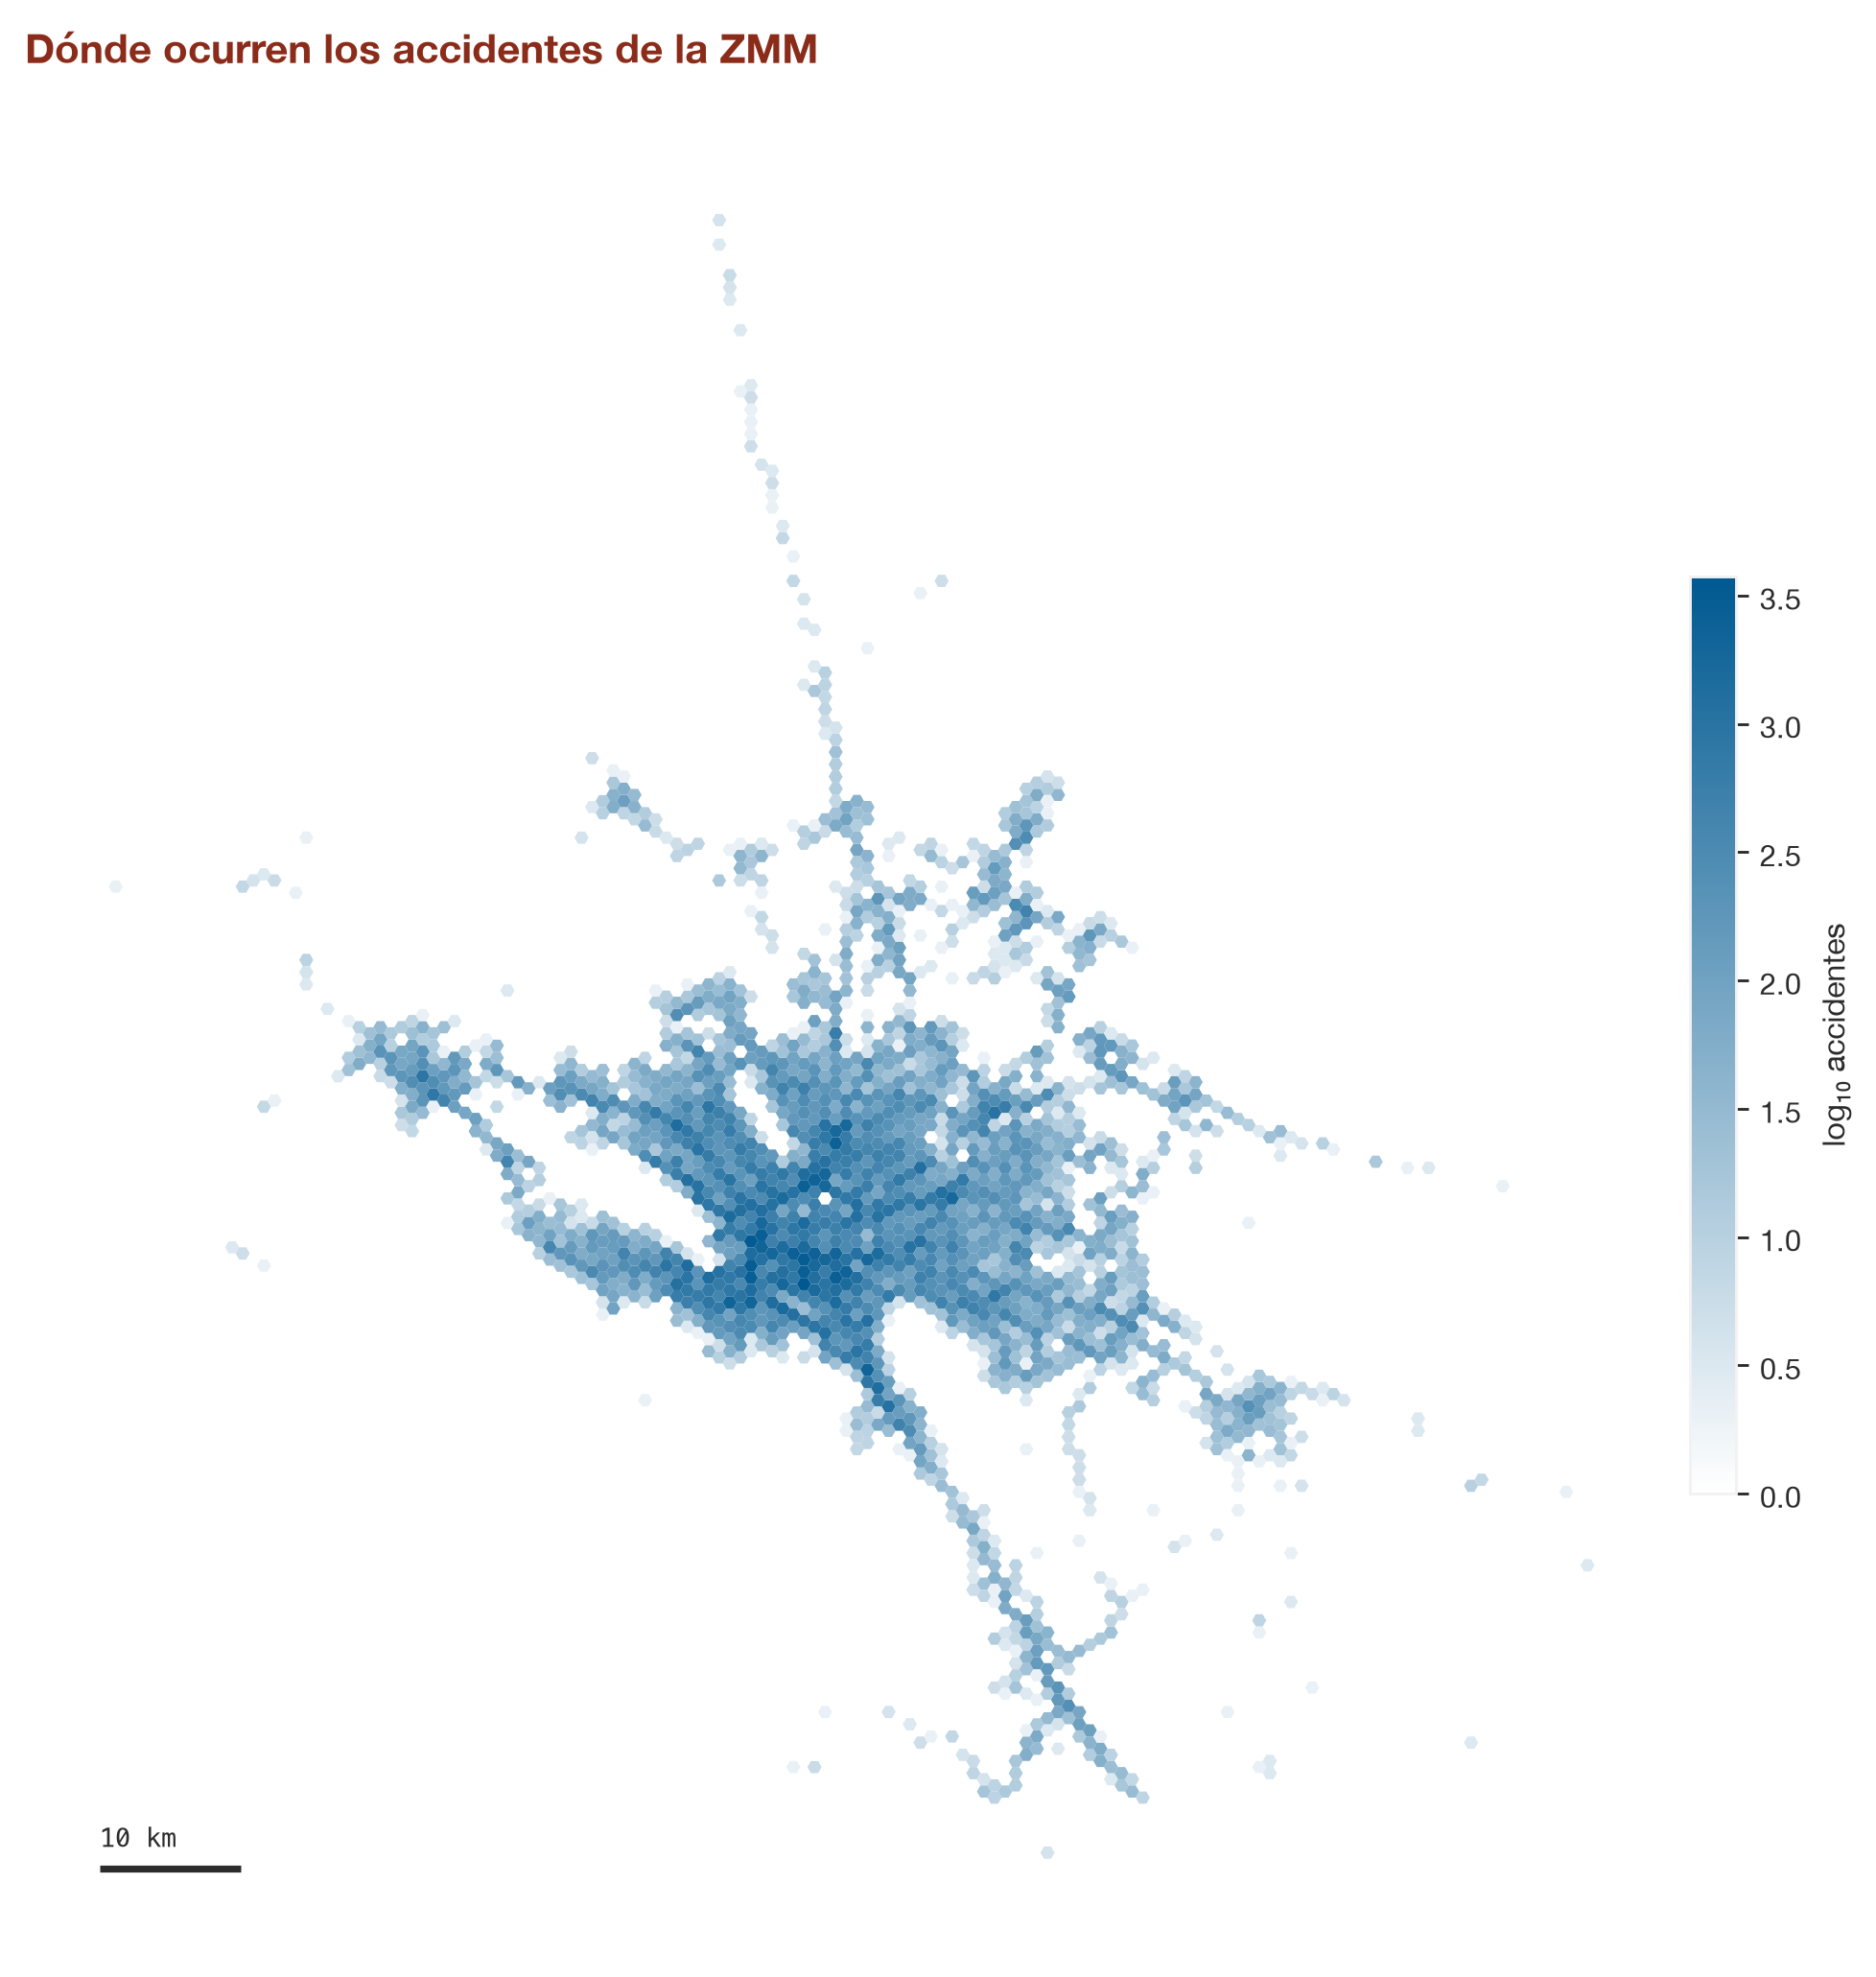
\includegraphics[width=0.78\textwidth]{conteos_hex}
\caption{Accidentes por celda hexagonal, 2019--2024, en escala logarítmica. La
mediana por celda es 30; el máximo, 3\,741.}
\end{figure}

\subsection{Autocorrelación global}

Con pesos de contigüidad estandarizados por fila y la variable $\log(1+n)$
(el conteo crudo tiene una cola que cinco celdas dominarían), el \textbf{$I$ de
Moran es 0,648}, con $z$ de permutación de 37 sobre 999 barajadas. Sobre el
conteo crudo es 0,57: la conclusión no depende de la transformación. Las
celdas no son independientes; un modelo que las trate así subestima sus
errores estándar.

\subsection{Sensibilidad a la escala}\label{sec:maup}

\begin{table}[H]
\centering\small
\begin{tabular}{rrrrrr}
\toprule
Lado (m) & Área (km$^2$) & Celdas & $I$ de Moran & Gini & Top 5\,\% concentra \\
\midrule
250   & 0,16 & 6\,145 & 0,524 & 0,746 & 44,8\,\% \\
500   & 0,65 & 2\,241 & 0,648 & 0,756 & 42,6\,\% \\
1\,000 & 2,60 & 815   & 0,721 & 0,788 & 43,5\,\% \\
\bottomrule
\end{tabular}
\caption{El $I$ de Moran crece con la agregación (efecto de escala esperado);
la concentración no cambia. La autocorrelación es una propiedad del fenómeno,
no de la rejilla.}
\end{table}

\subsection{Estructura local: LISA y $G^*$ de Getis--Ord}

Ambos estadísticos se calculan celda por celda con inferencia por
permutación. Con 2\,241 pruebas al 5\,\% se esperan $\sim$112 falsos positivos
por azar, así que se aplica corrección de Benjamini--Hochberg. El efecto es
material: \textbf{el LISA pasa de 682 celdas ``significativas'' a 287
($-58$\,\%)}, y el $G^*$ de 732 a 383. Sin corregir, casi la mitad del mapa de
puntos calientes sería ruido.

Lo que sobrevive: 266 celdas Alto--Alto que forman un núcleo compacto sobre la
mancha urbana consolidada, 17 Bajo--Bajo, y solo 4 atípicos espaciales. No hay
puntos calientes aislados: \emph{el riesgo es de corredor, no de esquina}. Las
303 celdas calientes del $G^*$ —el 13,5\,\% del territorio con red vial,
197\,km$^2$— concentran el 55\,\% de los accidentes.

\begin{figure}[H]
\centering
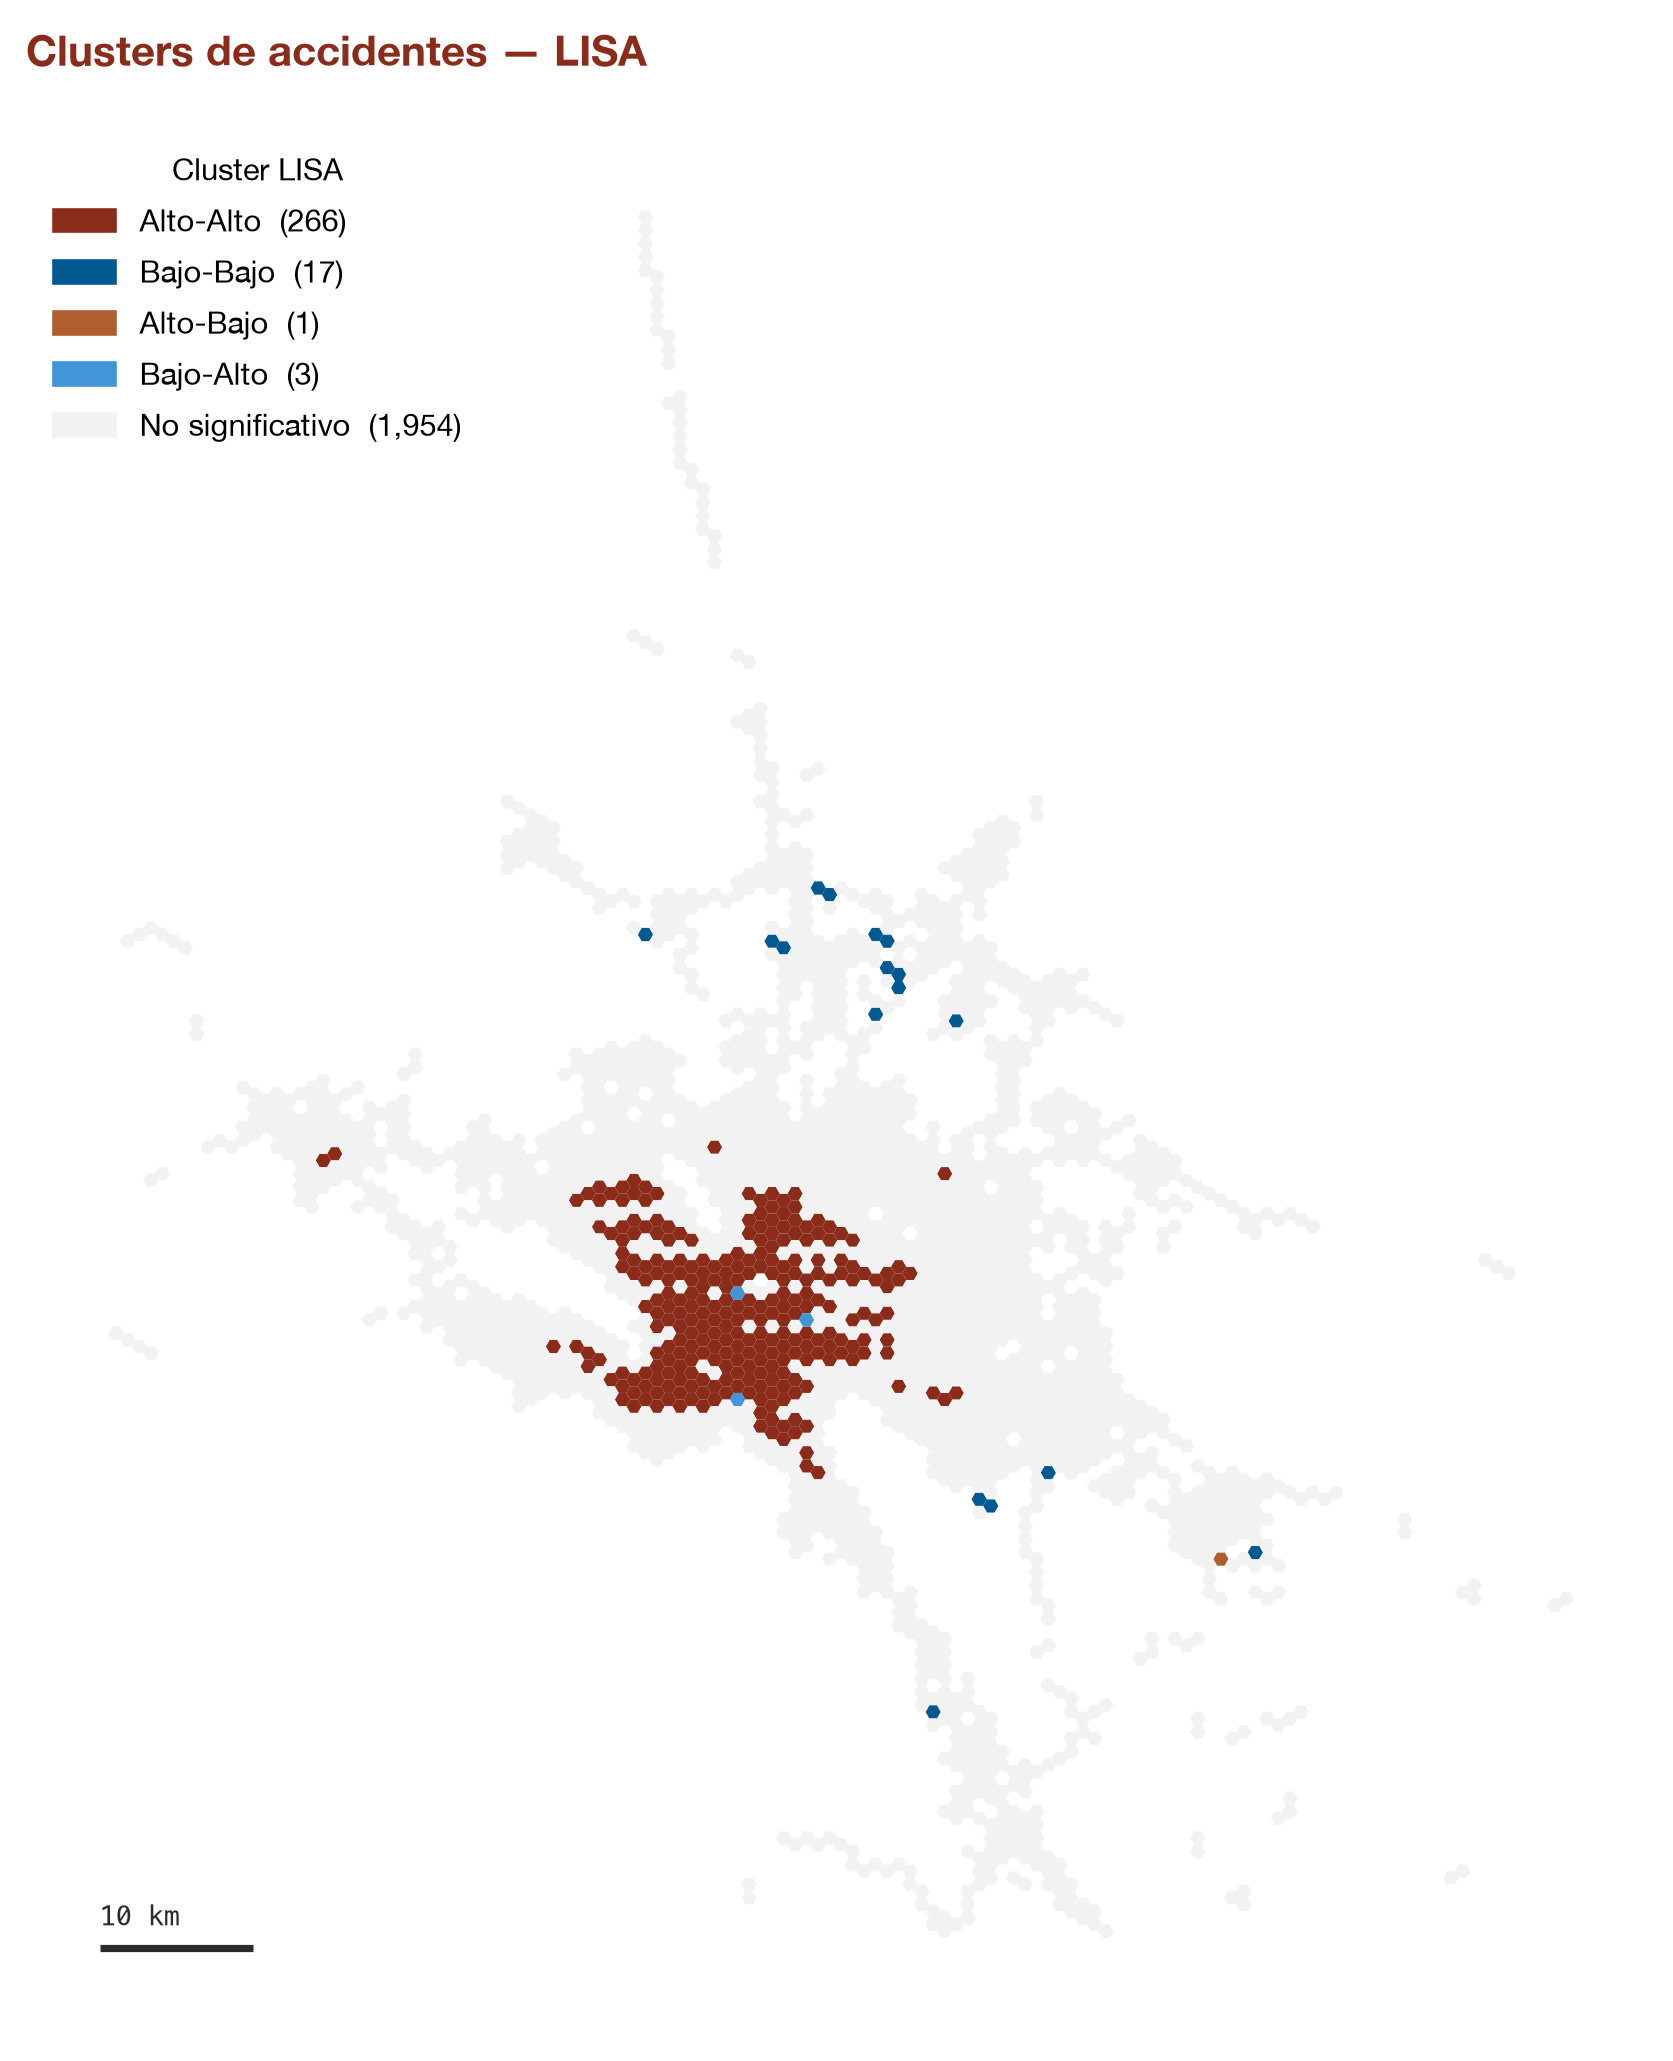
\includegraphics[width=0.48\textwidth]{lisa}\hfill
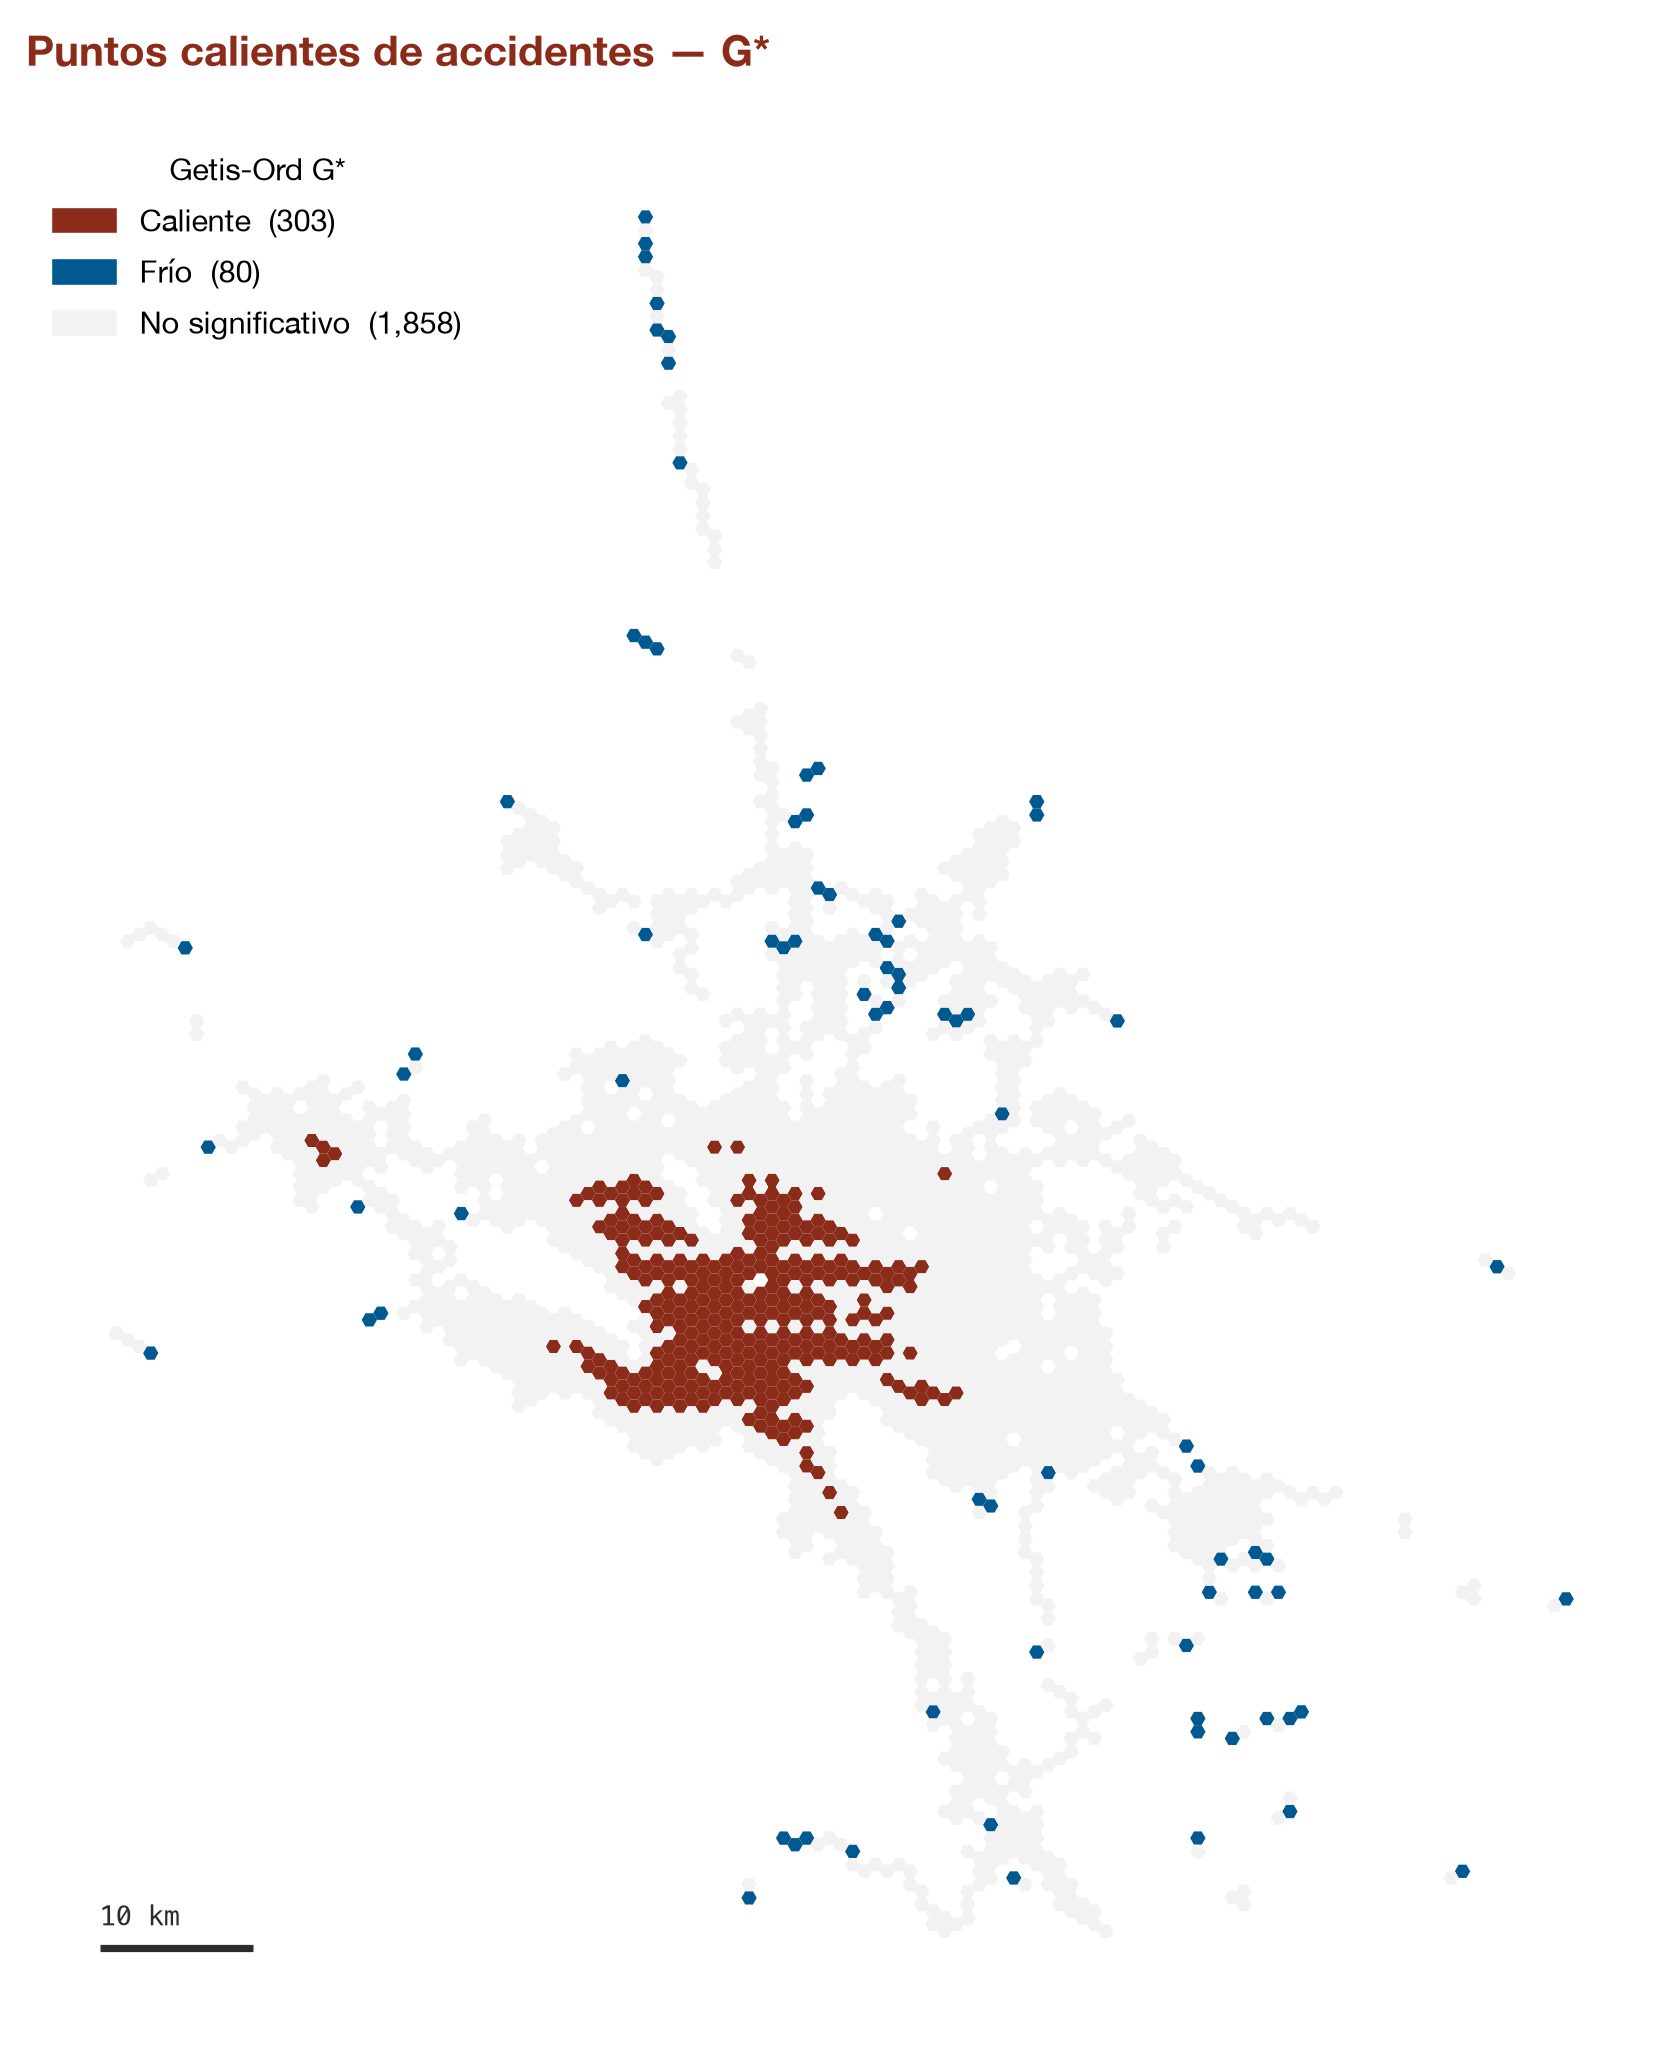
\includegraphics[width=0.48\textwidth]{gistar}
\caption{Izquierda: clusters LISA. Derecha: puntos calientes $G^*$. Ambos con
FDR al 5\,\%. Dos estadísticos con lógica distinta convergen en la misma
estructura.}
\end{figure}

\subsection{Persistencia: ¿el mapa de 2019 predice el de 2024?}

Es la sección que decide si el proyecto predictivo tiene sentido. El $I$ de
Moran se mantiene entre 0,60 y 0,69 los seis años, y el ranking de celdas de
2019 correlaciona \textbf{0,833 (Spearman) con el de 2024}, con una pandemia en
medio. La prueba operativa es el índice de precisión predictiva (PAI): la
fracción de accidentes capturada dividida entre la fracción de territorio
seleccionada. \textbf{Eligiendo el 5\,\% de las celdas con los datos de
2019--2023 se captura el 42\,\% de los accidentes de 2024: PAI 8,4.} Esto es sin
modelo —contar y ordenar— y es la cota que cualquier modelo tiene que superar.

\begin{figure}[H]
\centering
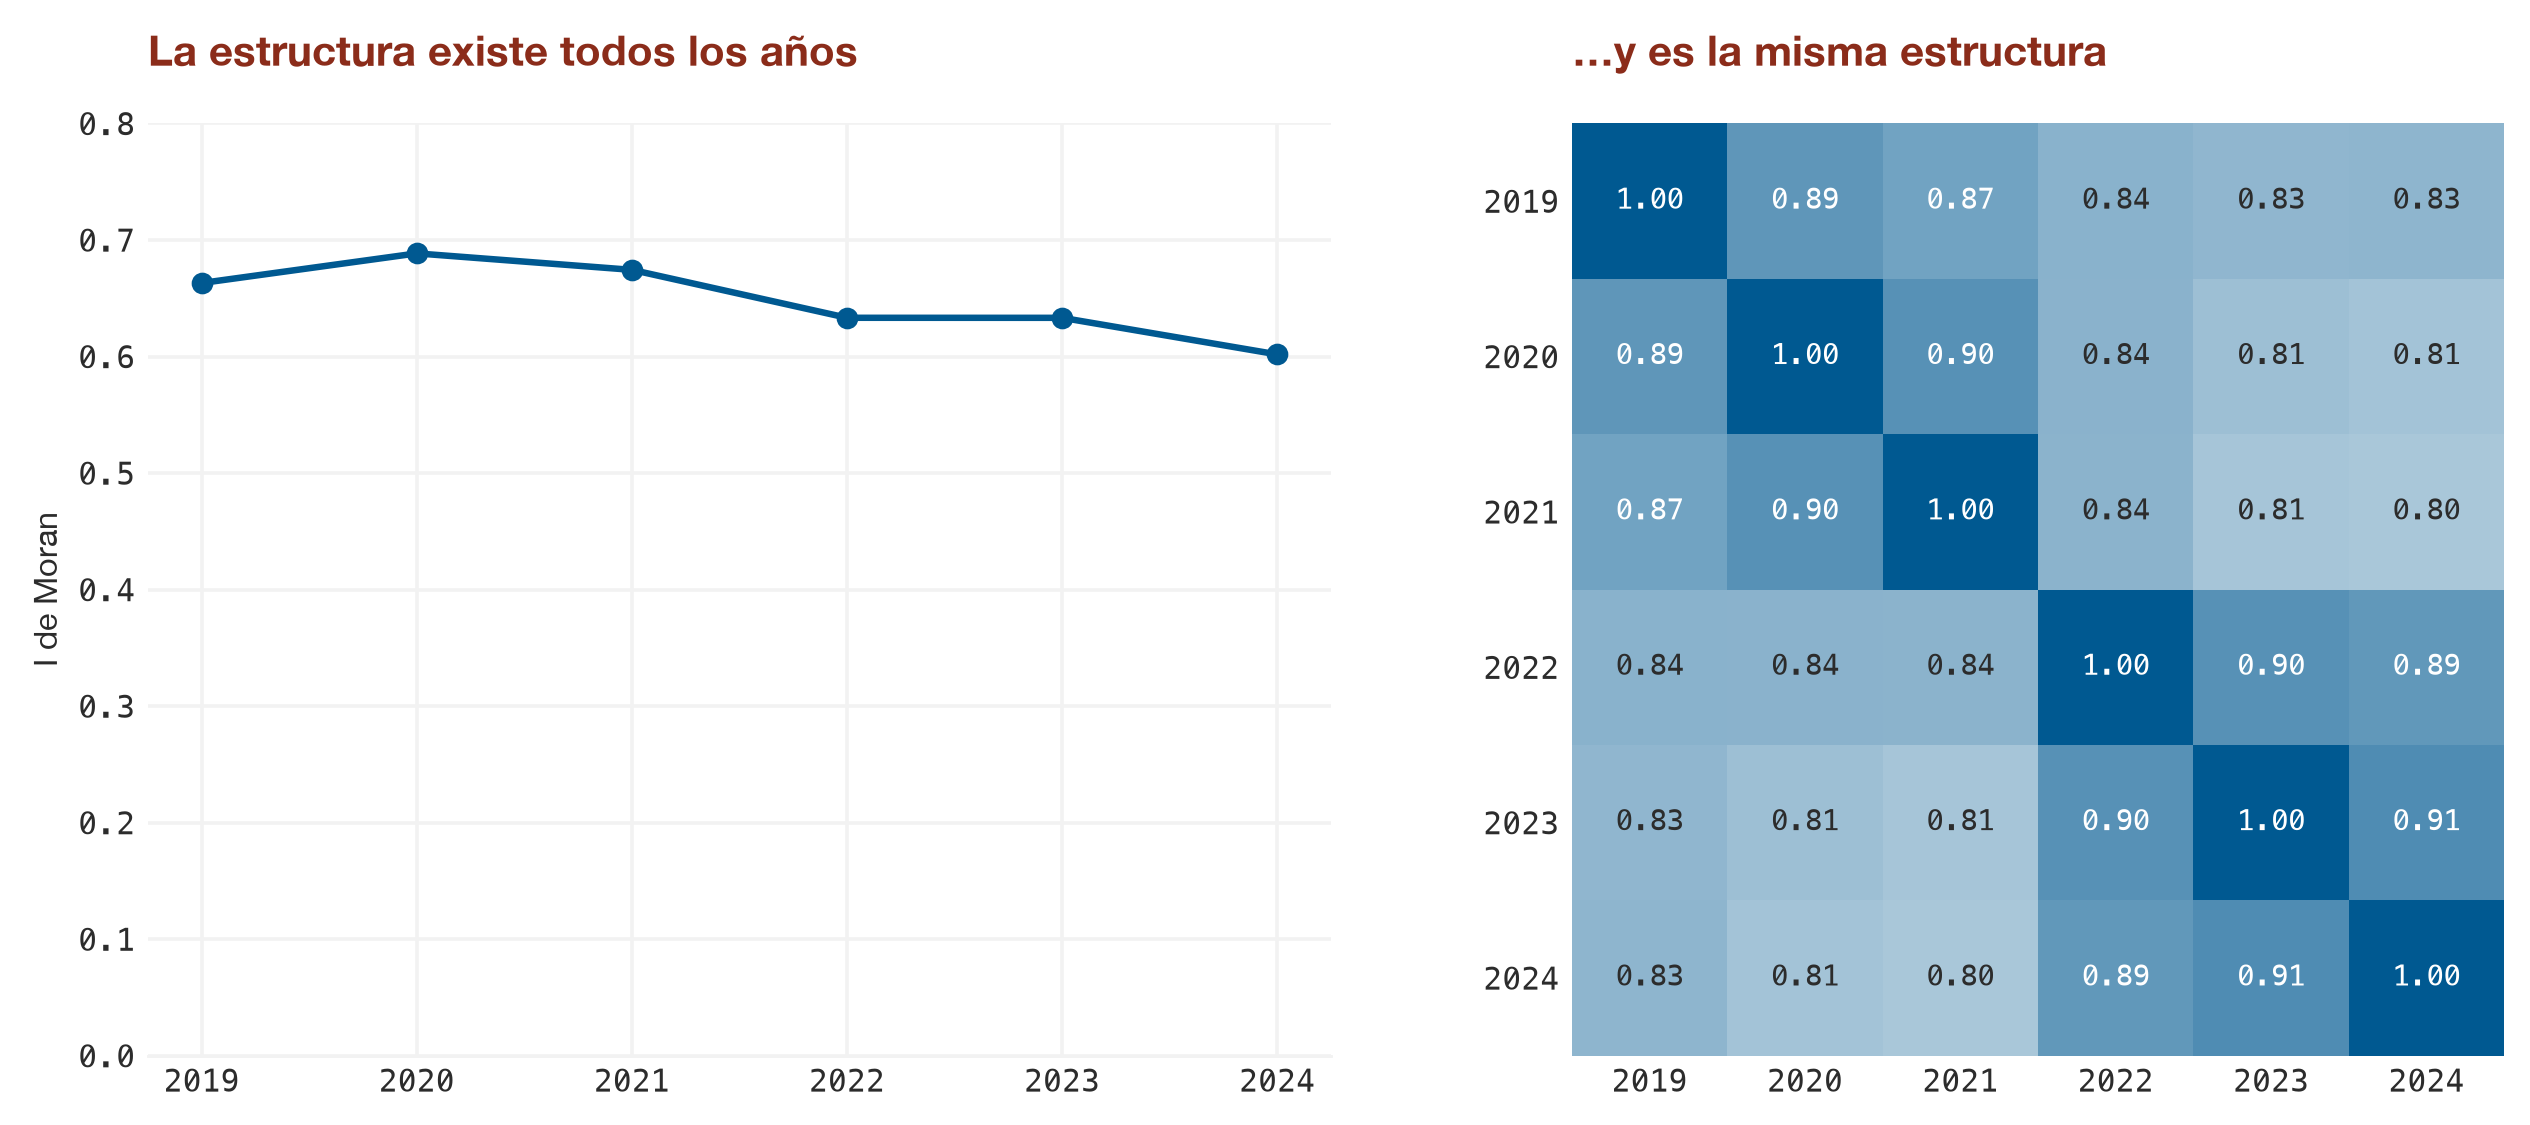
\includegraphics[width=0.95\textwidth]{persistencia}
\caption{Izquierda: $I$ de Moran por año. Derecha: Spearman entre los conteos
por celda de cada par de años. La matriz tiene dos bloques, 2019--2021 y
2022--2024.}
\end{figure}

\begin{advertencia}
\textbf{Hallazgo no previsto.} La matriz de Spearman tiene dos bloques
($\sim$0,90 dentro de 2019--2021 y de 2022--2024; $\sim$0,82 entre bloques).
Coincide con que el campo \texttt{OID} —el identificador que genera QGIS al
georreferenciar— solo existe en los archivos de 2022 en adelante. La hipótesis
más económica es un cambio en el procedimiento de georreferenciación del
INEGI. Se incorporó al modelo como indicador de periodo.
\end{advertencia}

\subsection{Lo que no se hizo}

La función $K$ de Ripley y la densidad kernel en sus versiones planas suponen
que un evento puede ocurrir en cualquier punto del plano; aquí solo puede
ocurrir sobre la red vial, y usarlas sobreestimaría el agrupamiento contra un
nulo imposible. Las versiones restringidas a red exigen la geometría de las
calles, que no está en el repositorio. Se decidió no correrlas: contestarían
una pregunta ya contestada (hay agrupamiento, y a qué escalas) a un costo alto.

% ===========================================================================
\section{Modelos de conteo}
% ===========================================================================

\subsection{El panel y el protocolo}

Panel de \textbf{2\,241 celdas $\times$ 72 meses $=$ 161\,352 filas}, con los
ceros explícitos (el 56\,\% de las filas). Entrenamiento 2019--2023, prueba
2024. Regla fijada desde el inicio: \emph{ningún modelo se compara en los datos
con que se ajustó}. Métricas: devianza de Poisson y MAE (¿acierta la media?),
CRPS y cobertura del intervalo del 90\,\% (¿acierta la distribución?), PAI
(¿sirve para elegir dónde intervenir?).

Covariables, todas estructurales: mes (factor), periodo (prepandemia /
pandemia / 2022 en adelante) y $\log h_i$, el promedio mensual histórico de la
celda calculado solo con entrenamiento. Su coeficiente es interpretable:
$\beta_h = 1$ significa que la historia entra como \emph{offset}; $\beta_h < 1$
significaría encogimiento hacia la media.

\subsection{Poisson y sobredispersión}

El GLM de Poisson se ajusta sabiendo que fallará, para documentar cómo. La
razón varianza/media del panel es 12,9 (marginal); condicionando en $\log h$
cae a $\chi^2_{\text{Pearson}}/gl = 1{,}38$: la historia de la celda absorbe
casi toda la heterogeneidad. Lo que queda es inequívoco: la prueba de
Cameron--Trivedi da $\hat\alpha = 0{,}096$ con $t = 59$.

\subsection{Binomial Negativa}

La mezcla Poisson--Gamma (NB2) con $\theta = 5{,}5$ corrige la varianza:
$\Var(Y) = \mu + \mu^2/\theta$. Supera a NB1 (varianza lineal) por 600 puntos
de AIC y a Poisson por 13\,000. La prueba de razón de verosimilitudes está en
la frontera del espacio paramétrico ($1/\theta = 0$), y su distribución nula
es una mezcla 50:50 de una masa en cero y una $\chi^2_1$; el $p$ correcto es la
mitad del de tabla. El rootograma colgante muestra el ajuste: Poisson
subpredice los ceros en 4\,500 y sobrepredice los unos en 2\,900; NB2 lo corrige
casi del todo.

\begin{figure}[H]
\centering
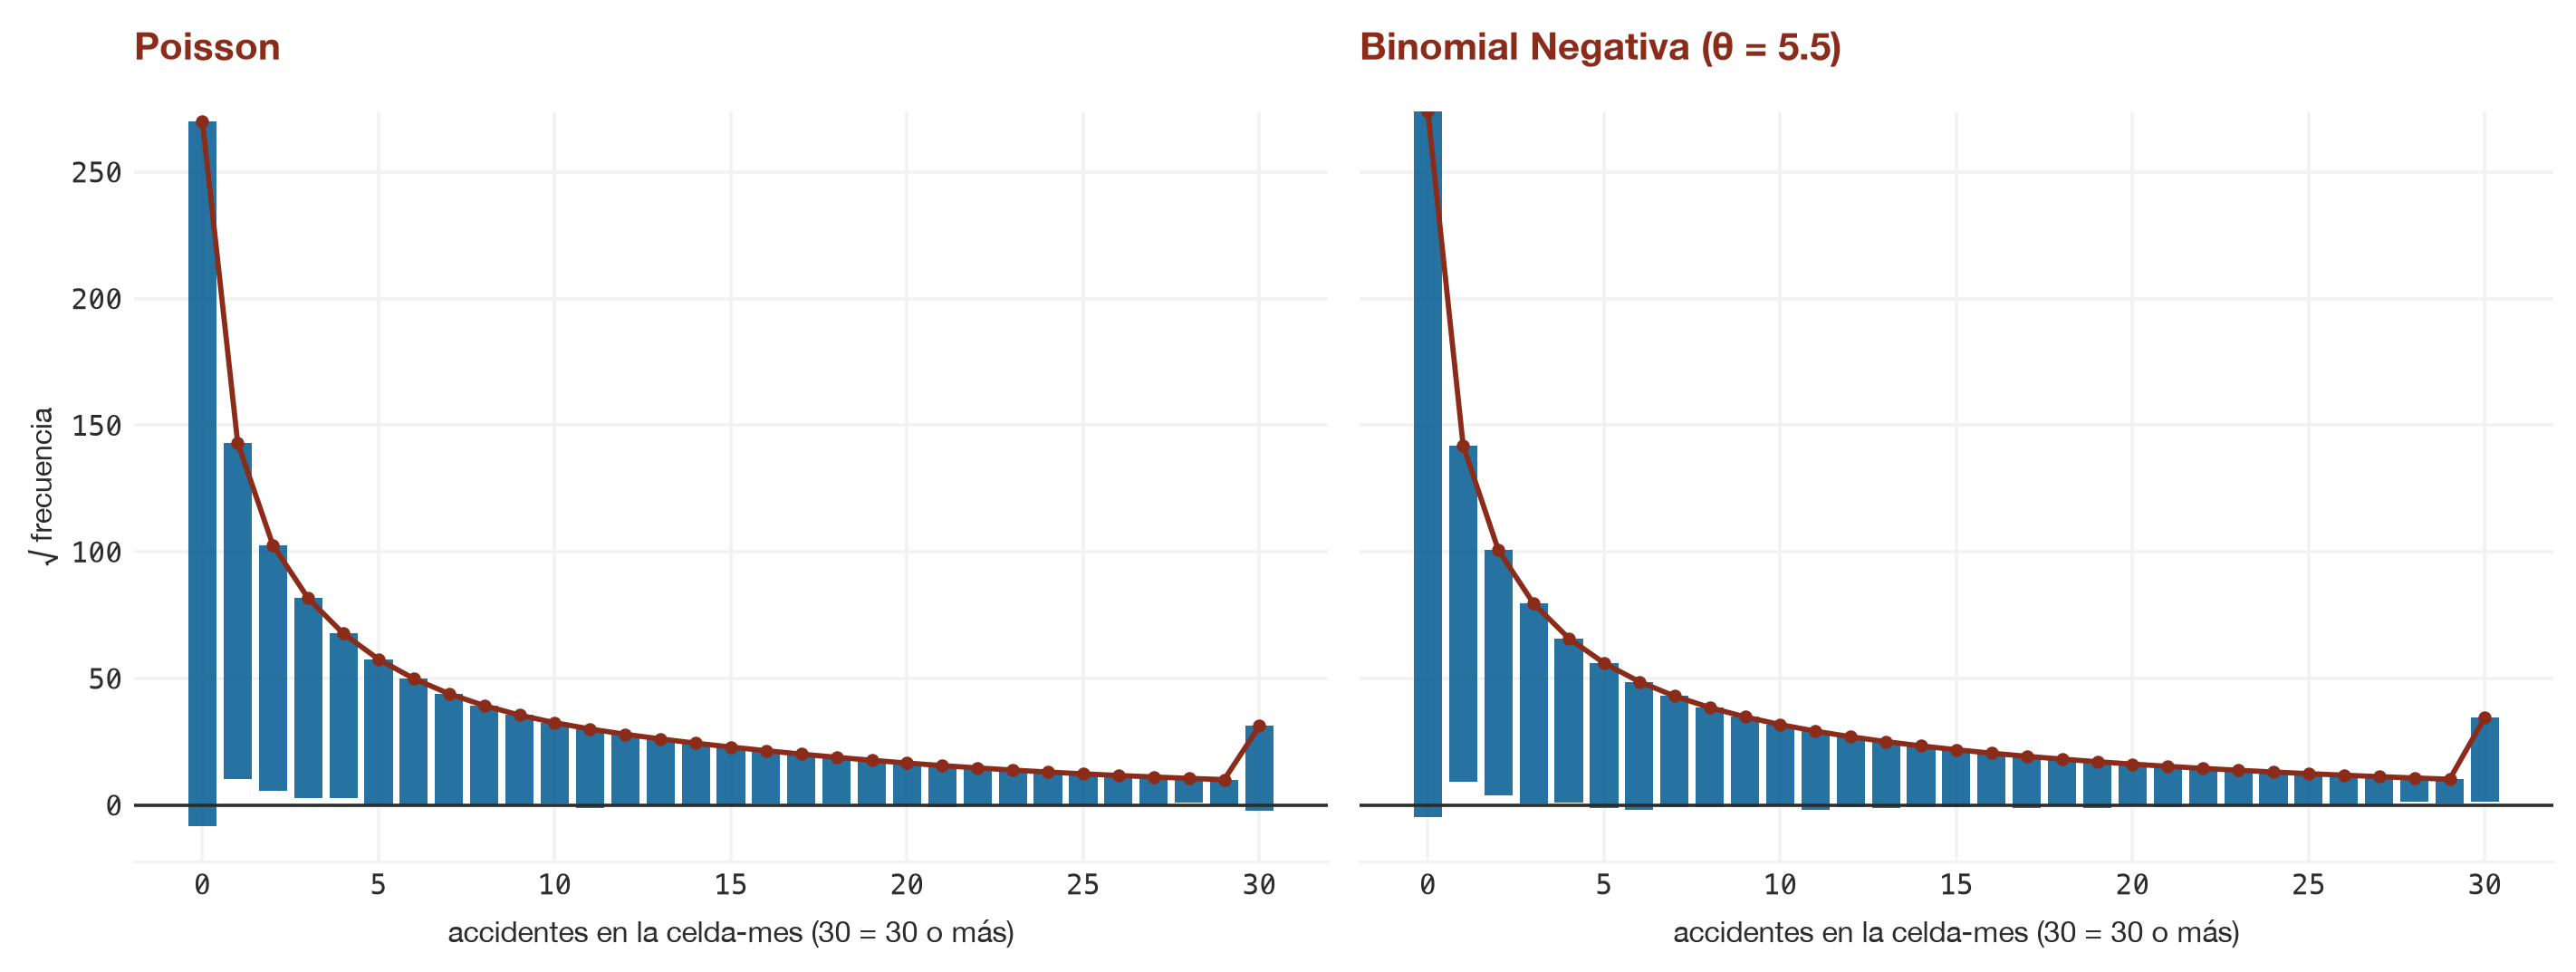
\includegraphics[width=0.95\textwidth]{rootograma}
\caption{Rootogramas colgantes. Las barras cuelgan de la frecuencia esperada;
si tocan el cero, el modelo ajusta ese valor.}
\end{figure}

\subsection{Ceros: por qué no ZINB}

A NB2 le faltan el 3,3\,\% de los ceros. Un ZINB con inflación constante
estima $\hat\pi = 0{,}026$ y mejora el AIC en 1\,200. Pero la pregunta útil no es
si ponerle un modelo sino \emph{de dónde salen}: ocho pares
municipio$\times$periodo explican dos tercios del exceso, con Santa Catarina
en prepandemia y pandemia a la cabeza. Ese municipio registró 128, 3 y 77
accidentes en 2019, 2020 y 2021, y 1\,793 en 2022. Los ceros ``estructurales''
son celdas cuyo municipio no reportaba, no celdas sin riesgo. Un ZINB con
inflación constante repartiría esa probabilidad entre todas las celdas por
igual: exactamente lo contrario de lo que pasa.

\begin{decision}{sin inflación de ceros}
El exceso de ceros es un fenómeno de régimen de reporte por municipio y se
modela como tal en la jerarquía, no como una segunda ecuación.
\end{decision}

\subsection{El resultado que reorganizó el proyecto}\label{sec:municipal}

\begin{table}[H]
\centering\small
\begin{tabular}{lrrrrr}
\toprule
Modelo (hex$\times$mes) & Devianza & MAE & CRPS & Cobertura 90\,\% & PAI 5\,\% \\
\midrule
M0 histórico 2019--23   & 40\,737 & 1,246 & 0,909 & 89,8\,\% & 8,41 \\
M0r histórico 2022--23  & 35\,652 & 1,196 & \textbf{0,844} & 92,0\,\% & 8,38 \\
M1 Poisson              & 39\,705 & 1,247 & 0,895 & 90,2\,\% & 8,41 \\
M2 NB2                  & 39\,701 & 1,254 & 0,886 & 93,9\,\% & 8,41 \\
M3 NB2 + rezago espacial & 39\,702 & 1,254 & 0,886 & 93,9\,\% & 8,41 \\
M4 NB2, historia 2022--23 & 35\,701 & 1,200 & 0,847 & 92,0\,\% & 8,38 \\
\bottomrule
\end{tabular}
\caption{Validación en 2024 a escala celda$\times$mes.}
\end{table}

Tres cosas se leen en la tabla y una cuarta se lee en el mapa:

\begin{enumerate}[leftmargin=1.4em]
\item \textbf{El PAI es idéntico en M0--M3.} No es coincidencia: con
  $\beta_h = 1{,}01$ y covariables que solo varían en el tiempo, la predicción
  de cada celda es $h_i$ por un factor común. El ranking es el del histórico
  (Spearman $= 1{,}000$). \emph{Un GLM con covariables temporales no puede mover
  el dónde}; solo el cuánto y el con qué certeza.
\item \textbf{El rezago espacial no aporta nada} (coeficiente $-0{,}002$,
  $t = -0{,}6$), pese a un Moran de 0,65 sobre los conteos.
\item \textbf{Dos años recientes predicen mejor que cinco} (CRPS 0,847 contra
  0,886). Y cuando el modelo recibe ambas historias elige la completa y
  pierde: en entrenamiento la historia larga explica mejor 2019--2021 porque
  los incluye. Es la razón de que el AIC no pueda comparar ventanas de
  historia y de que solo cuente la validación fuera de muestra.
\item \textbf{El residual tiene forma de municipio.} El $I$ de Moran del
  residual de NB2 es 0,31; al quitar la media por municipio cae a 0,07. No
  queda un proceso espacial fino que modelar: quedan 18 bloques con un nivel
  distinto cada uno. Por eso el rezago no ayudó: las vecinas de una celda de
  Guadalupe también están en Guadalupe y se equivocan igual.
\end{enumerate}

\begin{figure}[H]
\centering
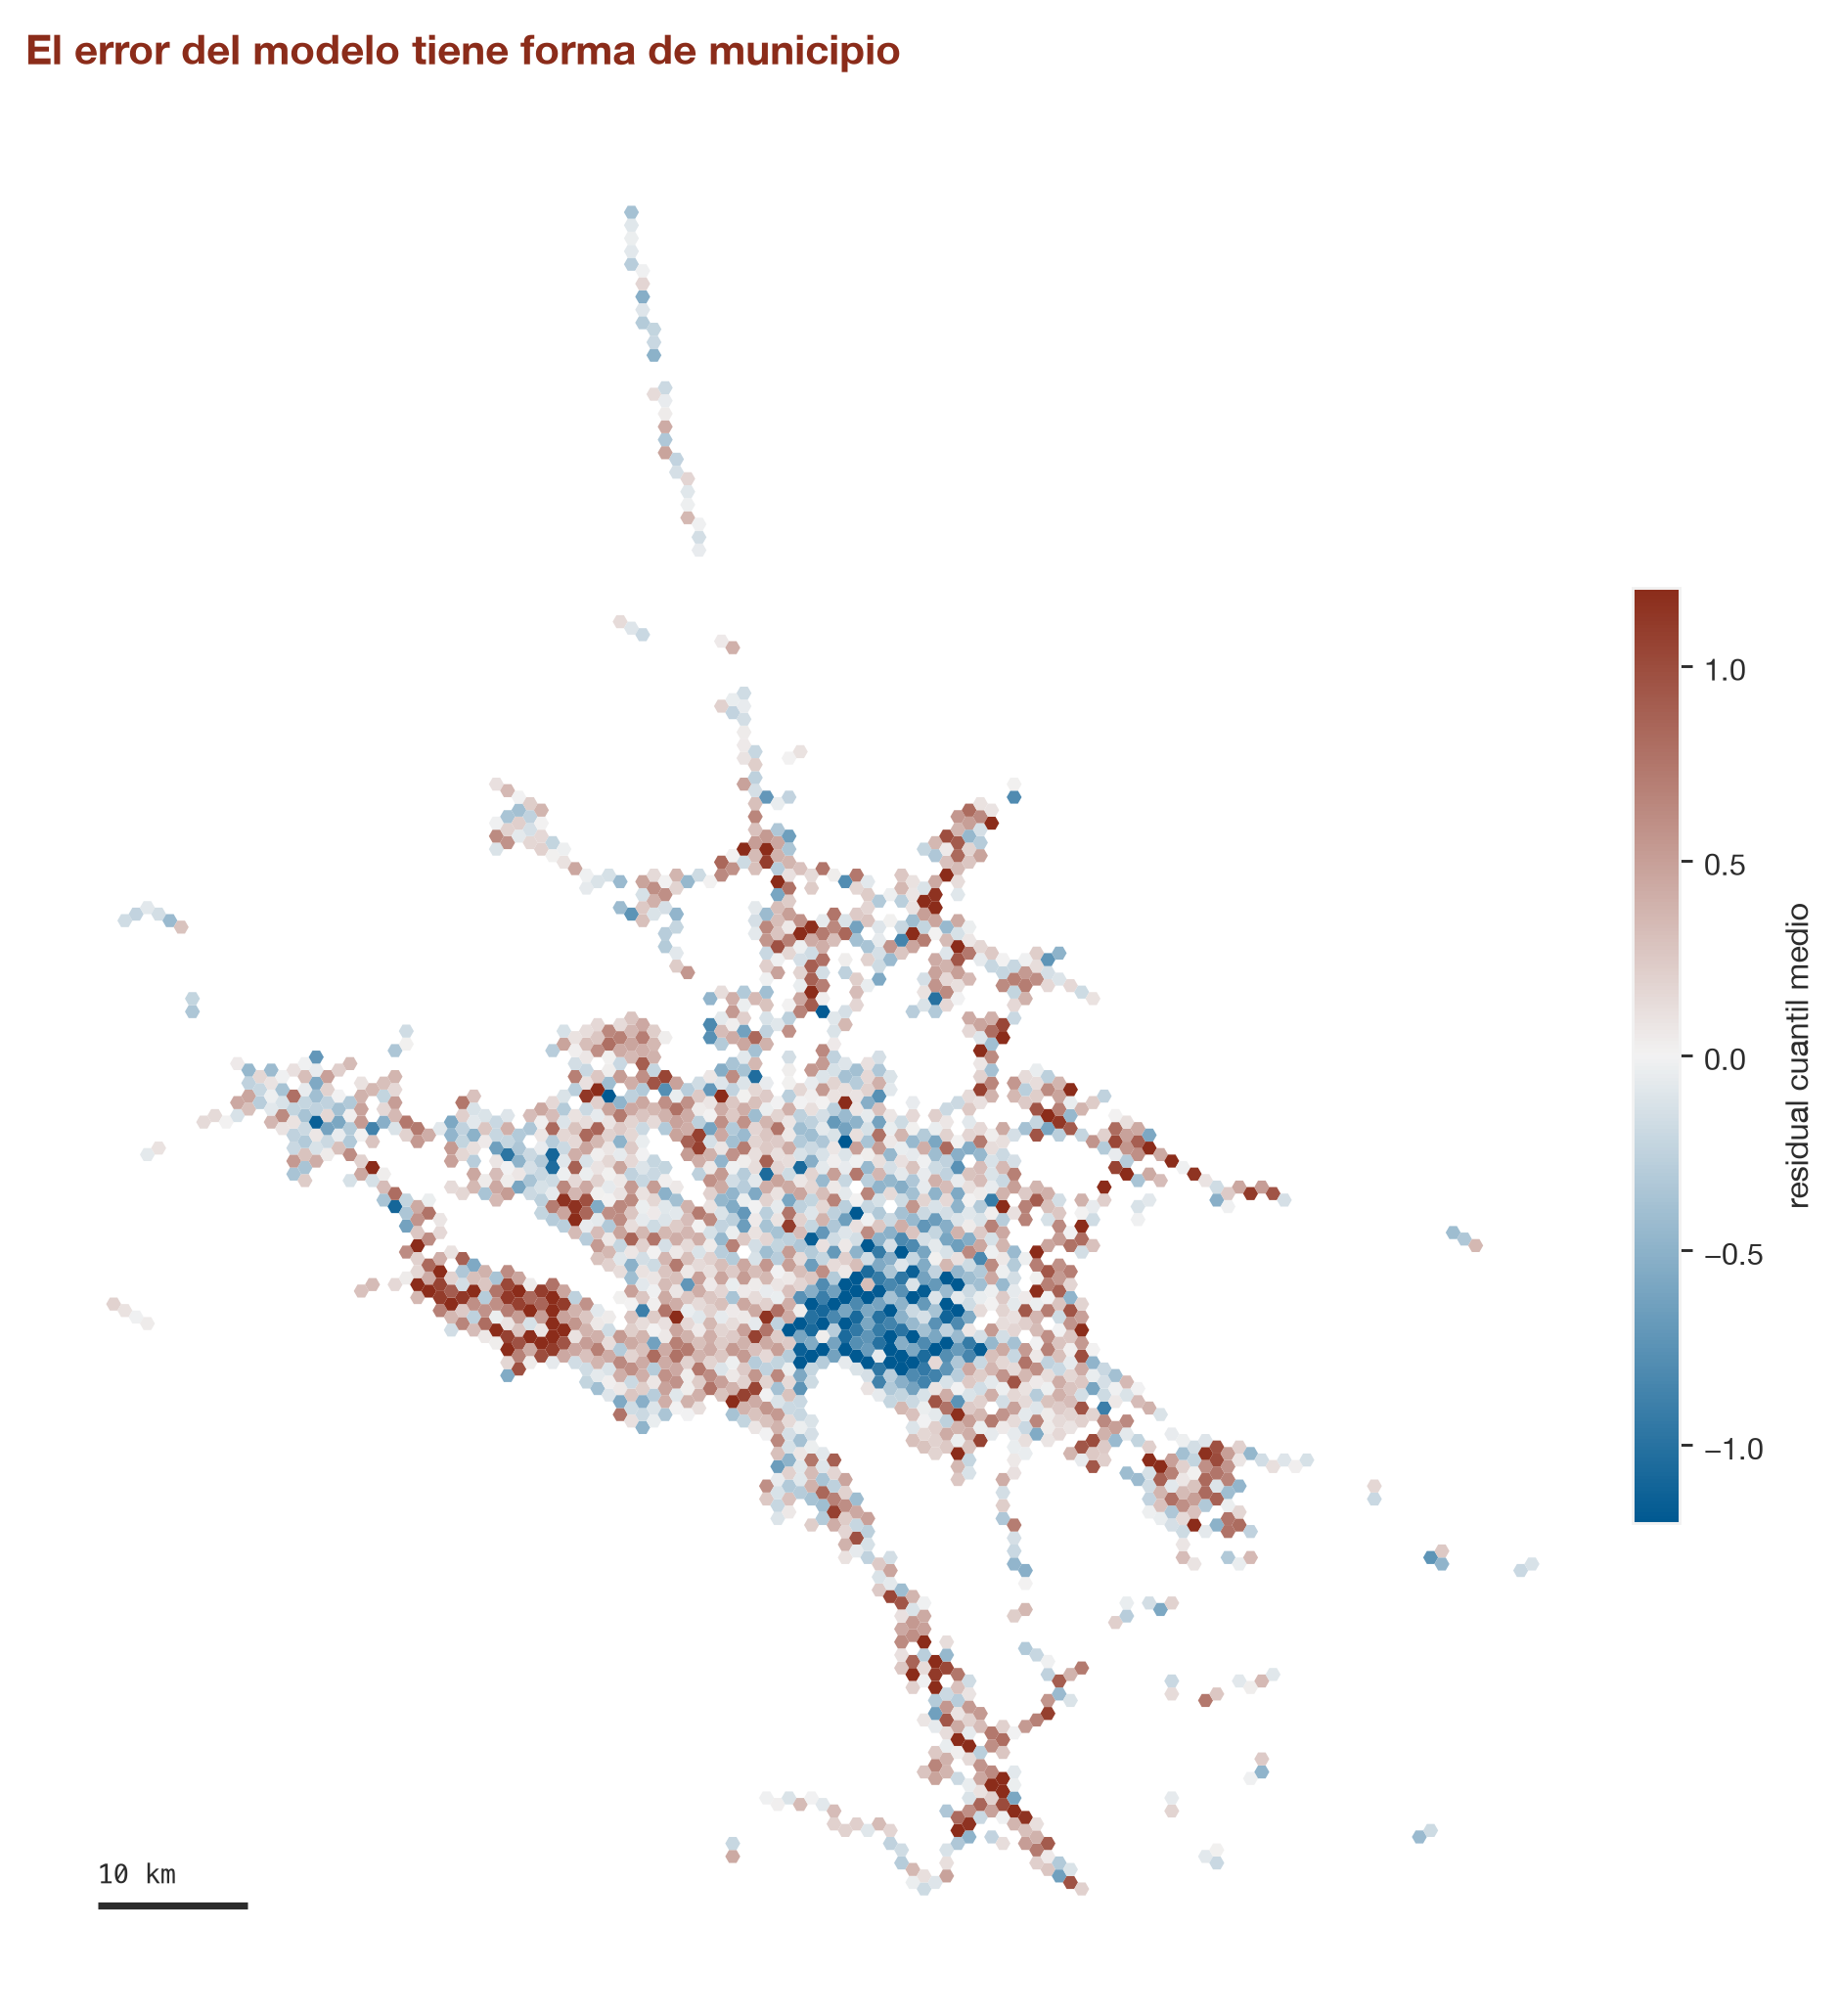
\includegraphics[width=0.48\textwidth]{residual_mapa}\hfill
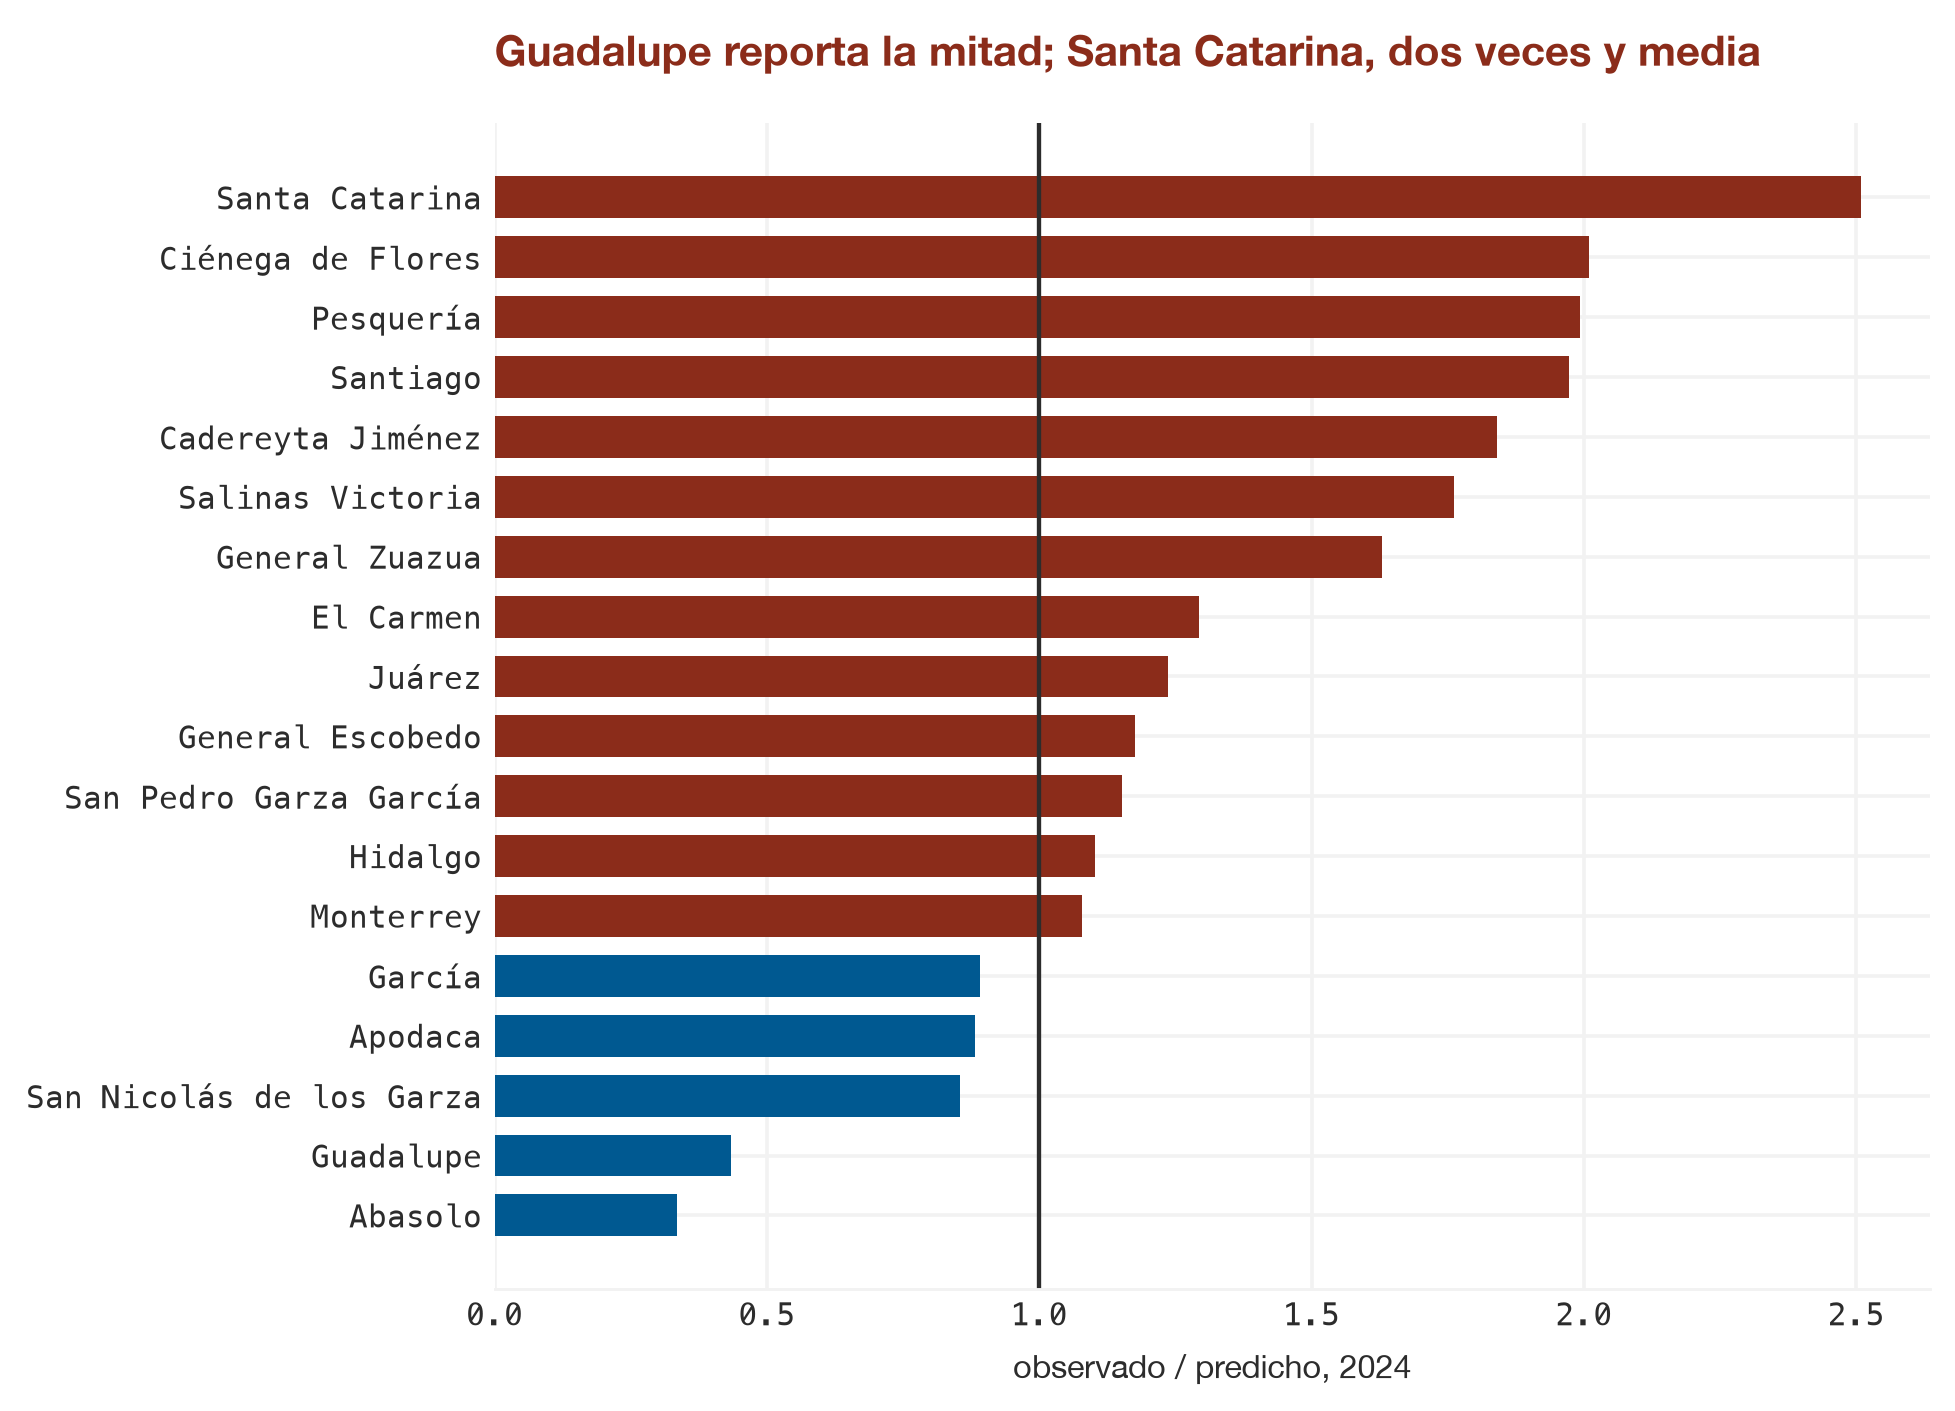
\includegraphics[width=0.48\textwidth]{cociente_municipal}
\caption{Izquierda: residual cuantil medio por celda en 2024 (NB2). Derecha:
cociente observado/predicho por municipio. Guadalupe tuvo el 43\,\% de lo que su
historia predice; Santa Catarina, 2,5 veces más.}
\end{figure}

\begin{figure}[H]
\centering
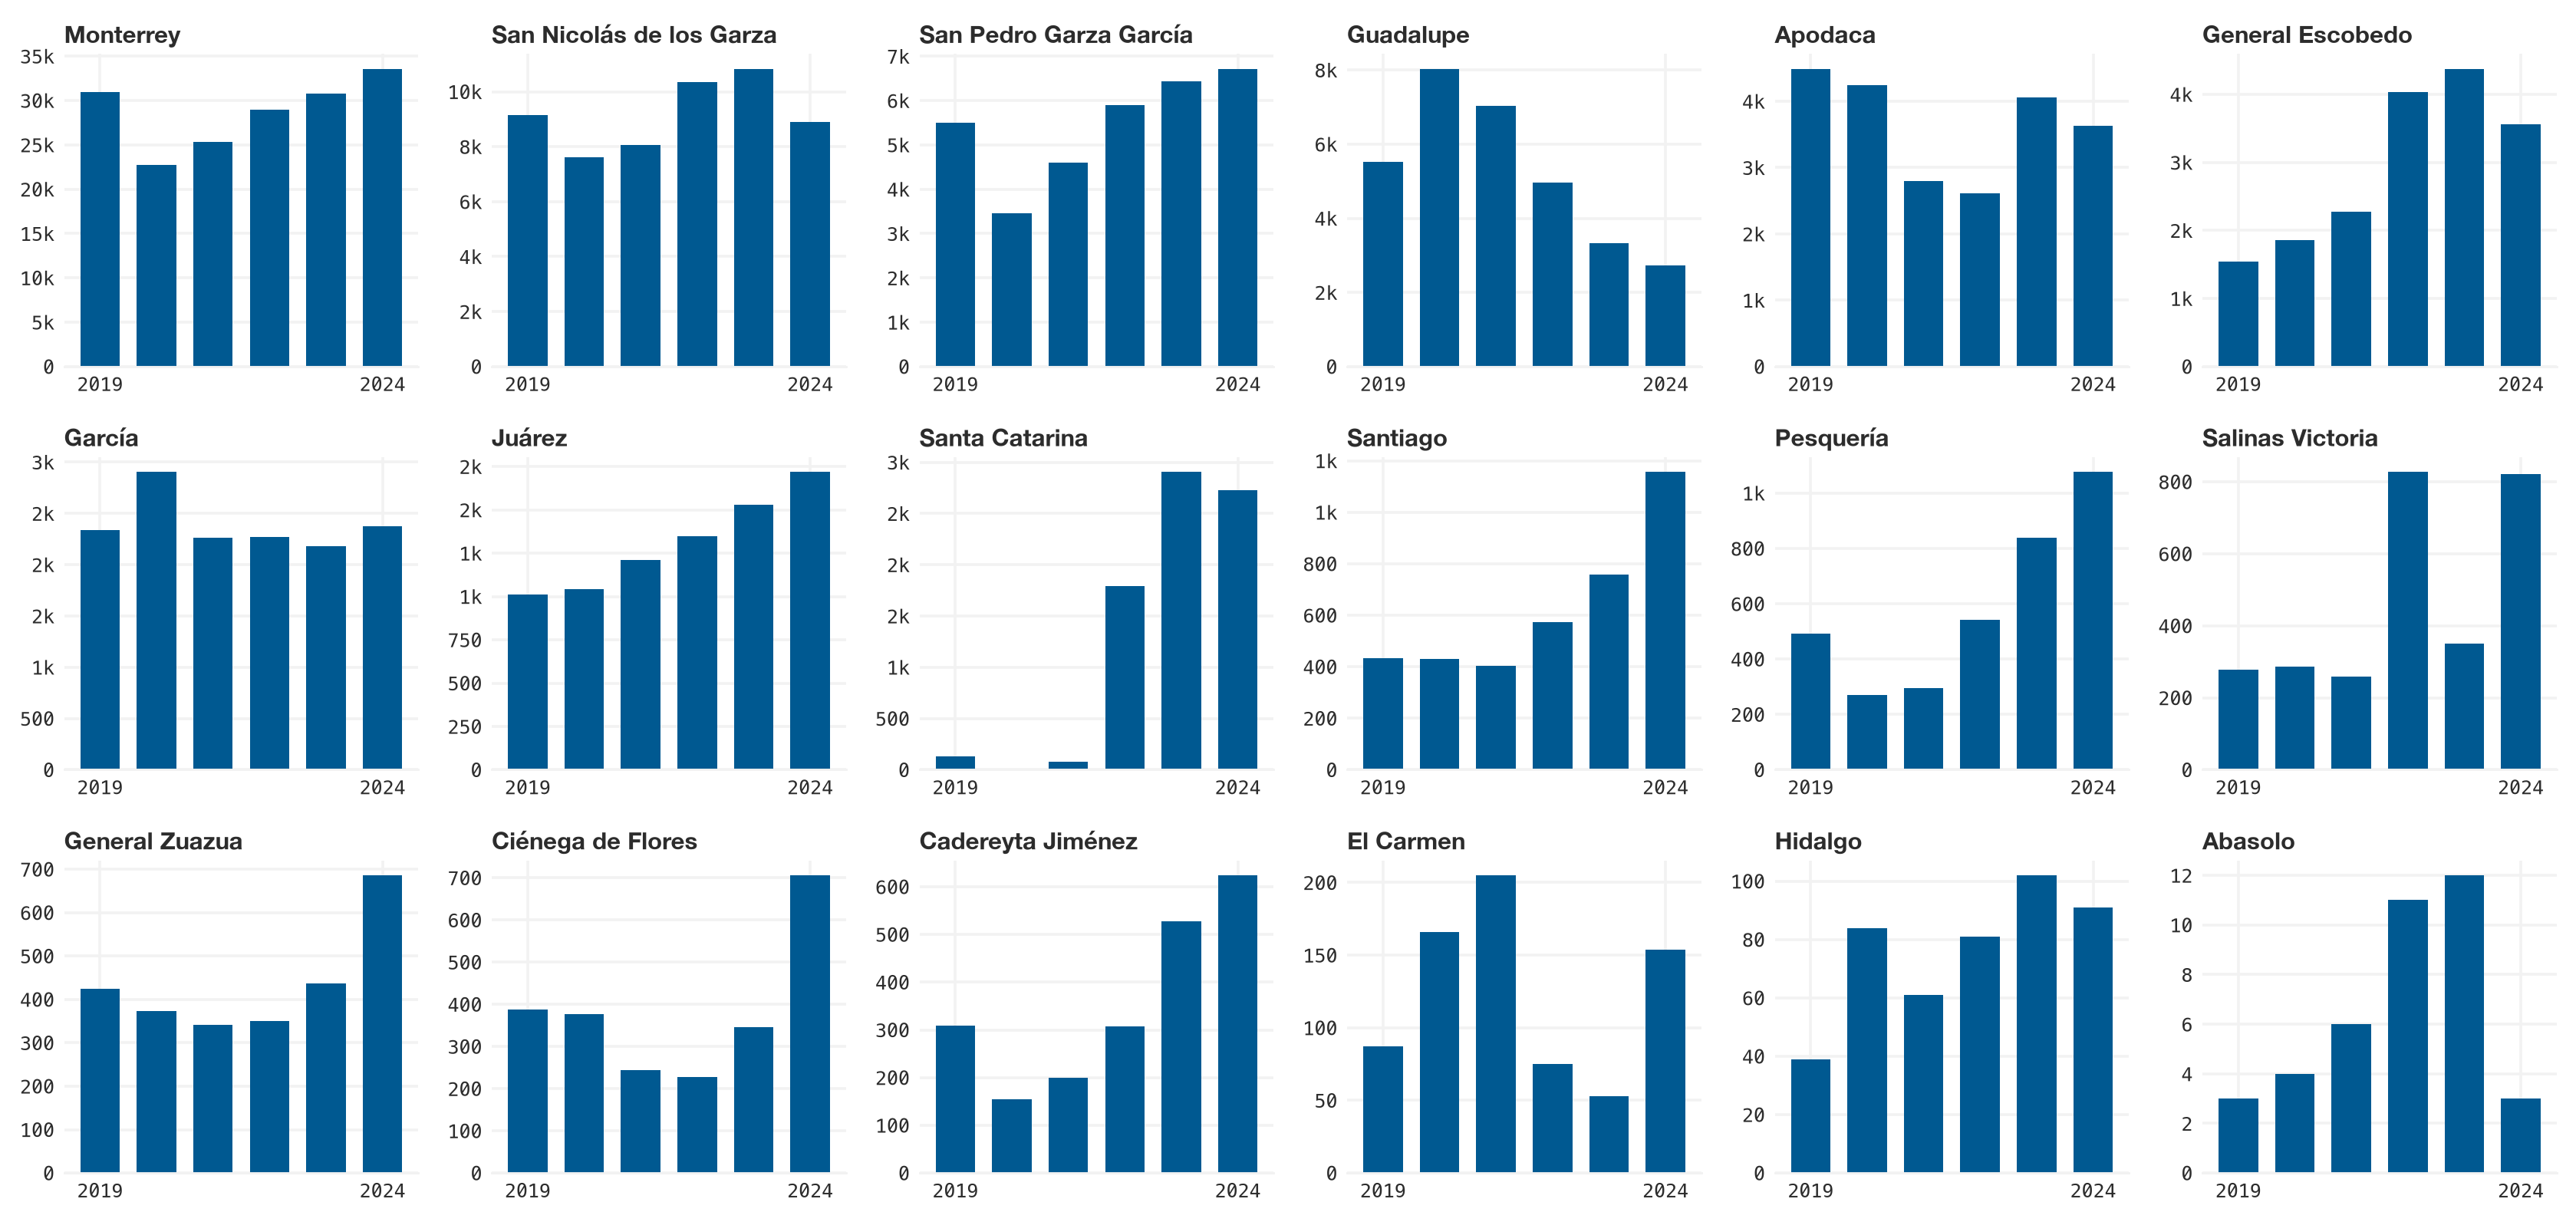
\includegraphics[width=0.98\textwidth]{series_municipales}
\caption{Accidentes registrados por año en cada municipio. Santa Catarina
registró 3 en 2020 y 2\,904 en 2023; Guadalupe alcanzó su máximo en plena
pandemia y cayó a un tercio en 2024; Salinas Victoria alterna 286, 827, 351,
821.}
\end{figure}

\begin{advertencia}
\textbf{El supuesto de subregistro estable es falso, y es la fuente dominante
del error.} Las series municipales no miden siniestralidad: miden la práctica
de captura de cada municipio cambiando de un año a otro. Cualquier modelo sobre
esta base es un modelo de \emph{reportes}. Esto se sabía cualitativamente por
la tasa de captura de \texttt{CINTURON} y \texttt{ALIENTO}; el conteo mismo lo
confirma con magnitudes que ninguna dinámica vial produce.
\end{advertencia}

% ===========================================================================
\section{El modelo jerárquico}
% ===========================================================================

\subsection{Especificación}

El notebook anterior decidió la especificación: Binomial Negativa, municipio
como nivel con efecto que cambia en el tiempo, y efecto espacial por celda
para el \emph{shrinkage}. Para la celda $i$, en el municipio $j(i)$, en el año $a$:
\begin{align}
Y_{ia} &\sim \NB(\mu_{ia},\ \theta), \\
\log \mu_{ia} &= \beta_0 + m_{j(i),a} + u_i .
\end{align}
El municipio absorbe \emph{cuánto se reporta}; la celda absorbe \emph{dónde,
dentro del municipio, se concentra}. Es la conclusión de
§\ref{sec:municipal} convertida en estructura.

\paragraph{Nivel municipal.} Caminata aleatoria con innovaciones de colas
pesadas:
\begin{equation}
m_{j,2019} = \sigma_m z_j,\quad z \sim \text{NormalSumaCero}(1); \qquad
m_{j,a} = m_{j,a-1} + \sigma_{rw}\,\varepsilon_{j,a},\quad \varepsilon \sim t_3 .
\end{equation}
La suma cero identifica $\beta_0$. Las innovaciones son $t$ y no normales por
lo que mostraron las series: la mayoría de los municipios se mueve poco y unos
pocos saltan. Con normales, $\sigma_{rw}$ salía 0,61 (inflado por los saltos);
con $t_3$, 0,29.

\paragraph{Nivel de celda.} CAR propio:
\begin{equation}
\mathbf{u} \sim \mathcal{N}\!\left(\mathbf{0},\ \sigma_u^2 (D - \alpha A)^{-1}\right),
\end{equation}
con $A$ la adyacencia de los hexágonos, $D$ la diagonal de grados y
$\alpha \in (0,1)$ la dependencia espacial.

\paragraph{Panel anual.} El modelo se ajusta sobre celda$\times$año (11\,205
filas de entrenamiento) y no celda$\times$mes. El efecto de mes es común a
todas las celdas y aportó casi nada sobre un promedio bien elegido (M4 $\approx$
M0r); toda la estructura de interés vive en el nivel anual. Es el supuesto de
separabilidad espacio-tiempo, apoyado por el Spearman de 0,83 entre años. Y
NUTS sobre 161 mil observaciones con 2\,300 parámetros tarda horas; sobre 11
mil, minutos.

\subsection{Por qué CAR propio y no BYM2}

La propuesta original era BYM2, $u_i = \sigma(\sqrt{1-\phi}\,v_i + \sqrt{\phi}\,s_i)$,
con $v$ independiente, $s$ ICAR y $\phi$ interpretable como fracción
espacial. Se intentó en las dos parametrizaciones y no se identificó:

\begin{table}[H]
\centering\small
\begin{tabular}{lll}
\toprule
Parametrización & Resultado & $\Rhat$ de $\phi$ \\
\midrule
No centrada & $\phi \to 0{,}0001$: la parte espacial desaparece & 2,06 \\
Centrada    & $\sigma_s \to 13$, $\phi \to 0{,}9998$: la parte independiente desaparece & 1,65 \\
\bottomrule
\end{tabular}
\end{table}

El motivo es de estructura, no de \emph{tuning}. Con cinco años de conteos por
celda, los datos fijan cada $u_i$ casi por completo; la descomposición en
``espacial'' e ``independiente'' solo la sostienen los priors, y el muestreador
cae en el modo degenerado más cercano. La estructura espacial \emph{existe}
—el Moran de la tasa por celda tras quitar la media municipal es 0,41—; lo
que no existe es información para repartirla entre dos componentes. El CAR
propio tiene una sola varianza y un solo $\alpha$, es un prior propio y se
identifica con datos fuertes.

\subsection{Ajuste y diagnósticos}

Cuatro cadenas NUTS (\texttt{nutpie}), 1\,000 iteraciones de calentamiento y
2\,000 muestras, en 4 minutos. \textbf{Cero divergencias}; sobre las 11\,205
cantidades $\log\mu_{ia}$ —que son las identificadas— el $\Rhat$ máximo es
1,005 y el ESS mínimo 2\,441. $\beta_0$ y $\sigma_m$ mezclan peor porque
comparten información con el nivel medio de $\mathbf{u}$; no se usan solos en
ninguna conclusión.

\begin{table}[H]
\centering\small
\begin{tabular}{lrrl}
\toprule
Parámetro & Media & IC 94\,\% & Lectura \\
\midrule
$\alpha$       & 0,85 & [0,81; 0,88] & Dependencia espacial fuerte, neta del municipio \\
$\theta$       & 12,2 &              & Sobredispersión moderada a escala anual (5,5 a escala mensual) \\
$\sigma_{rw}$  & 0,29 &              & El municipio típico cambia $\times 1{,}34$ al año \\
$\sigma_u$     & 2,38 &              & Las celdas difieren en órdenes de magnitud dentro del municipio \\
\bottomrule
\end{tabular}
\caption{Hiperparámetros a posteriori. Con priors alternativos ($\alpha$
uniforme, $\sigma_u$ el doble de ancho, $\theta$ con media 5 en vez de 20) los
cuatro cambian en el tercer decimal: los datos dominan.}
\end{table}

\begin{figure}[H]
\centering
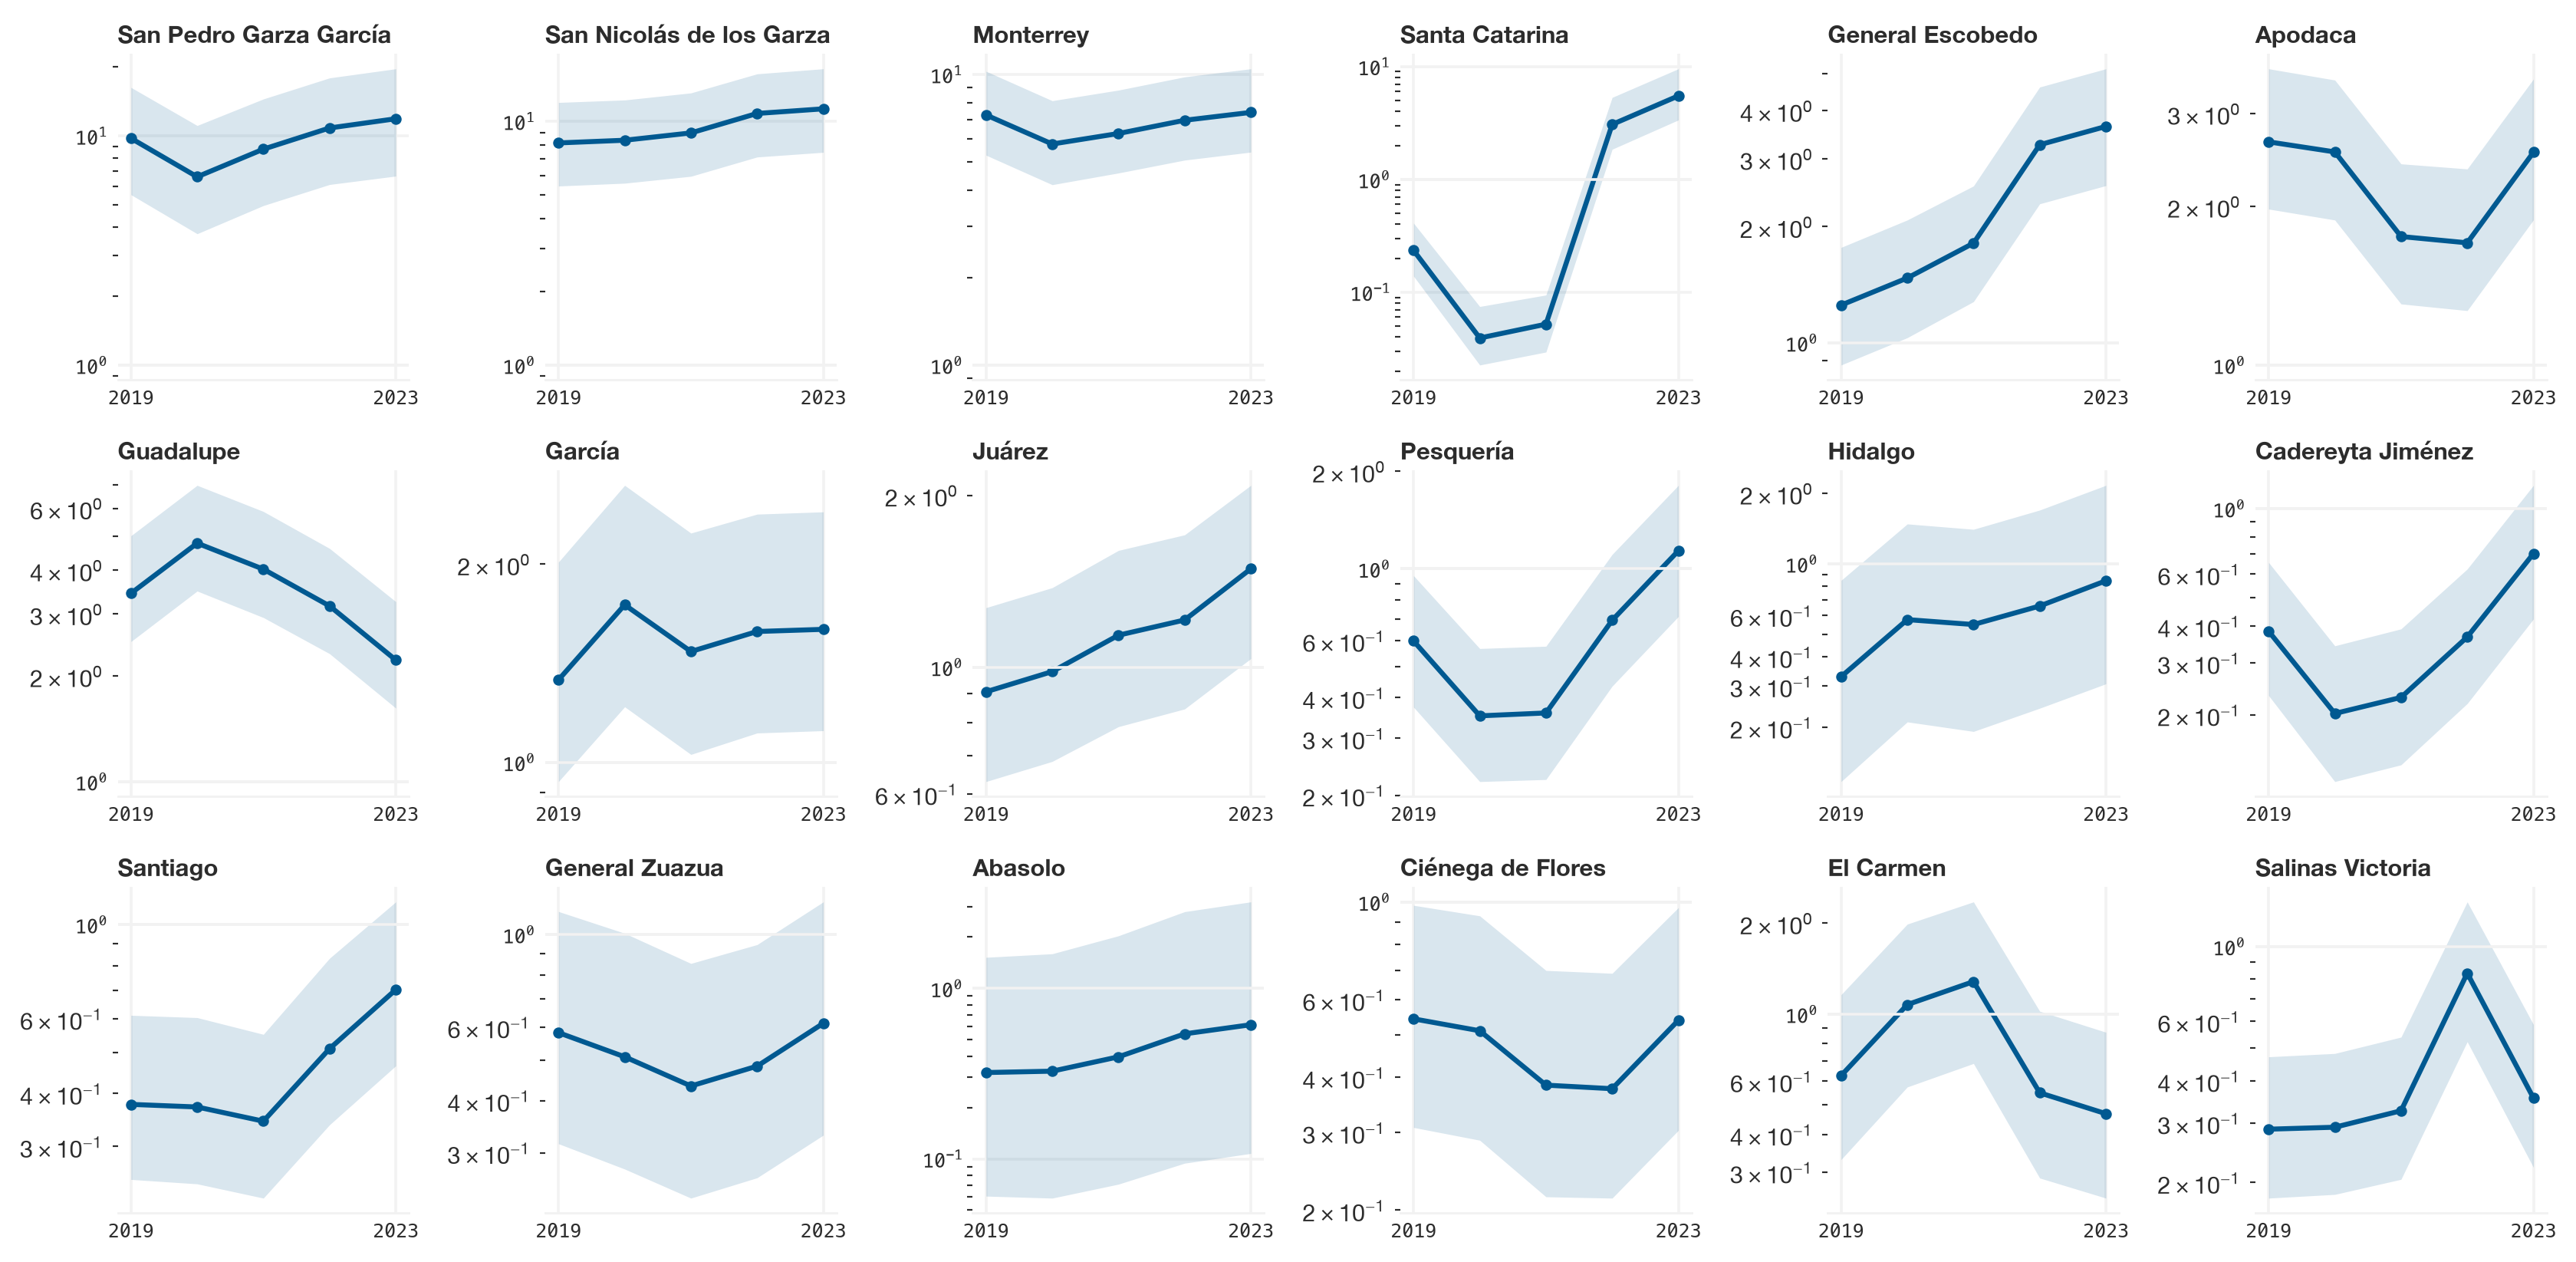
\includegraphics[width=0.98\textwidth]{trayectorias}
\caption{Efecto municipal $m_{j,a}$ a posteriori (mediana e intervalo del
90\,\%), en escala multiplicativa. Cada panel es un régimen de reporte; el
intervalo es angosto en los municipios grandes y ancho en los pequeños.}
\end{figure}

\subsection{El producto: el perfil espacial neto del municipio}

$u_i$ es cuánto más o menos riesgo tiene cada celda que el promedio de su
municipio, estimado con la información de la celda \emph{y} de sus vecinas.
En las 618 celdas con cinco accidentes o menos en cinco años, el modelo encoge
poco la estimación puntual (12\,\%) —el prior es ancho y deja hablar a los
datos— pero \textbf{triplica la incertidumbre} respecto a las celdas con más de
cien (0,75 contra 0,25 en escala log). Es el \emph{shrinkage} proporcional a la
ignorancia que motivó el enfoque: dos celdas con el mismo $u_i$ y distinta
incertidumbre no merecen la misma intervención.

\begin{figure}[H]
\centering
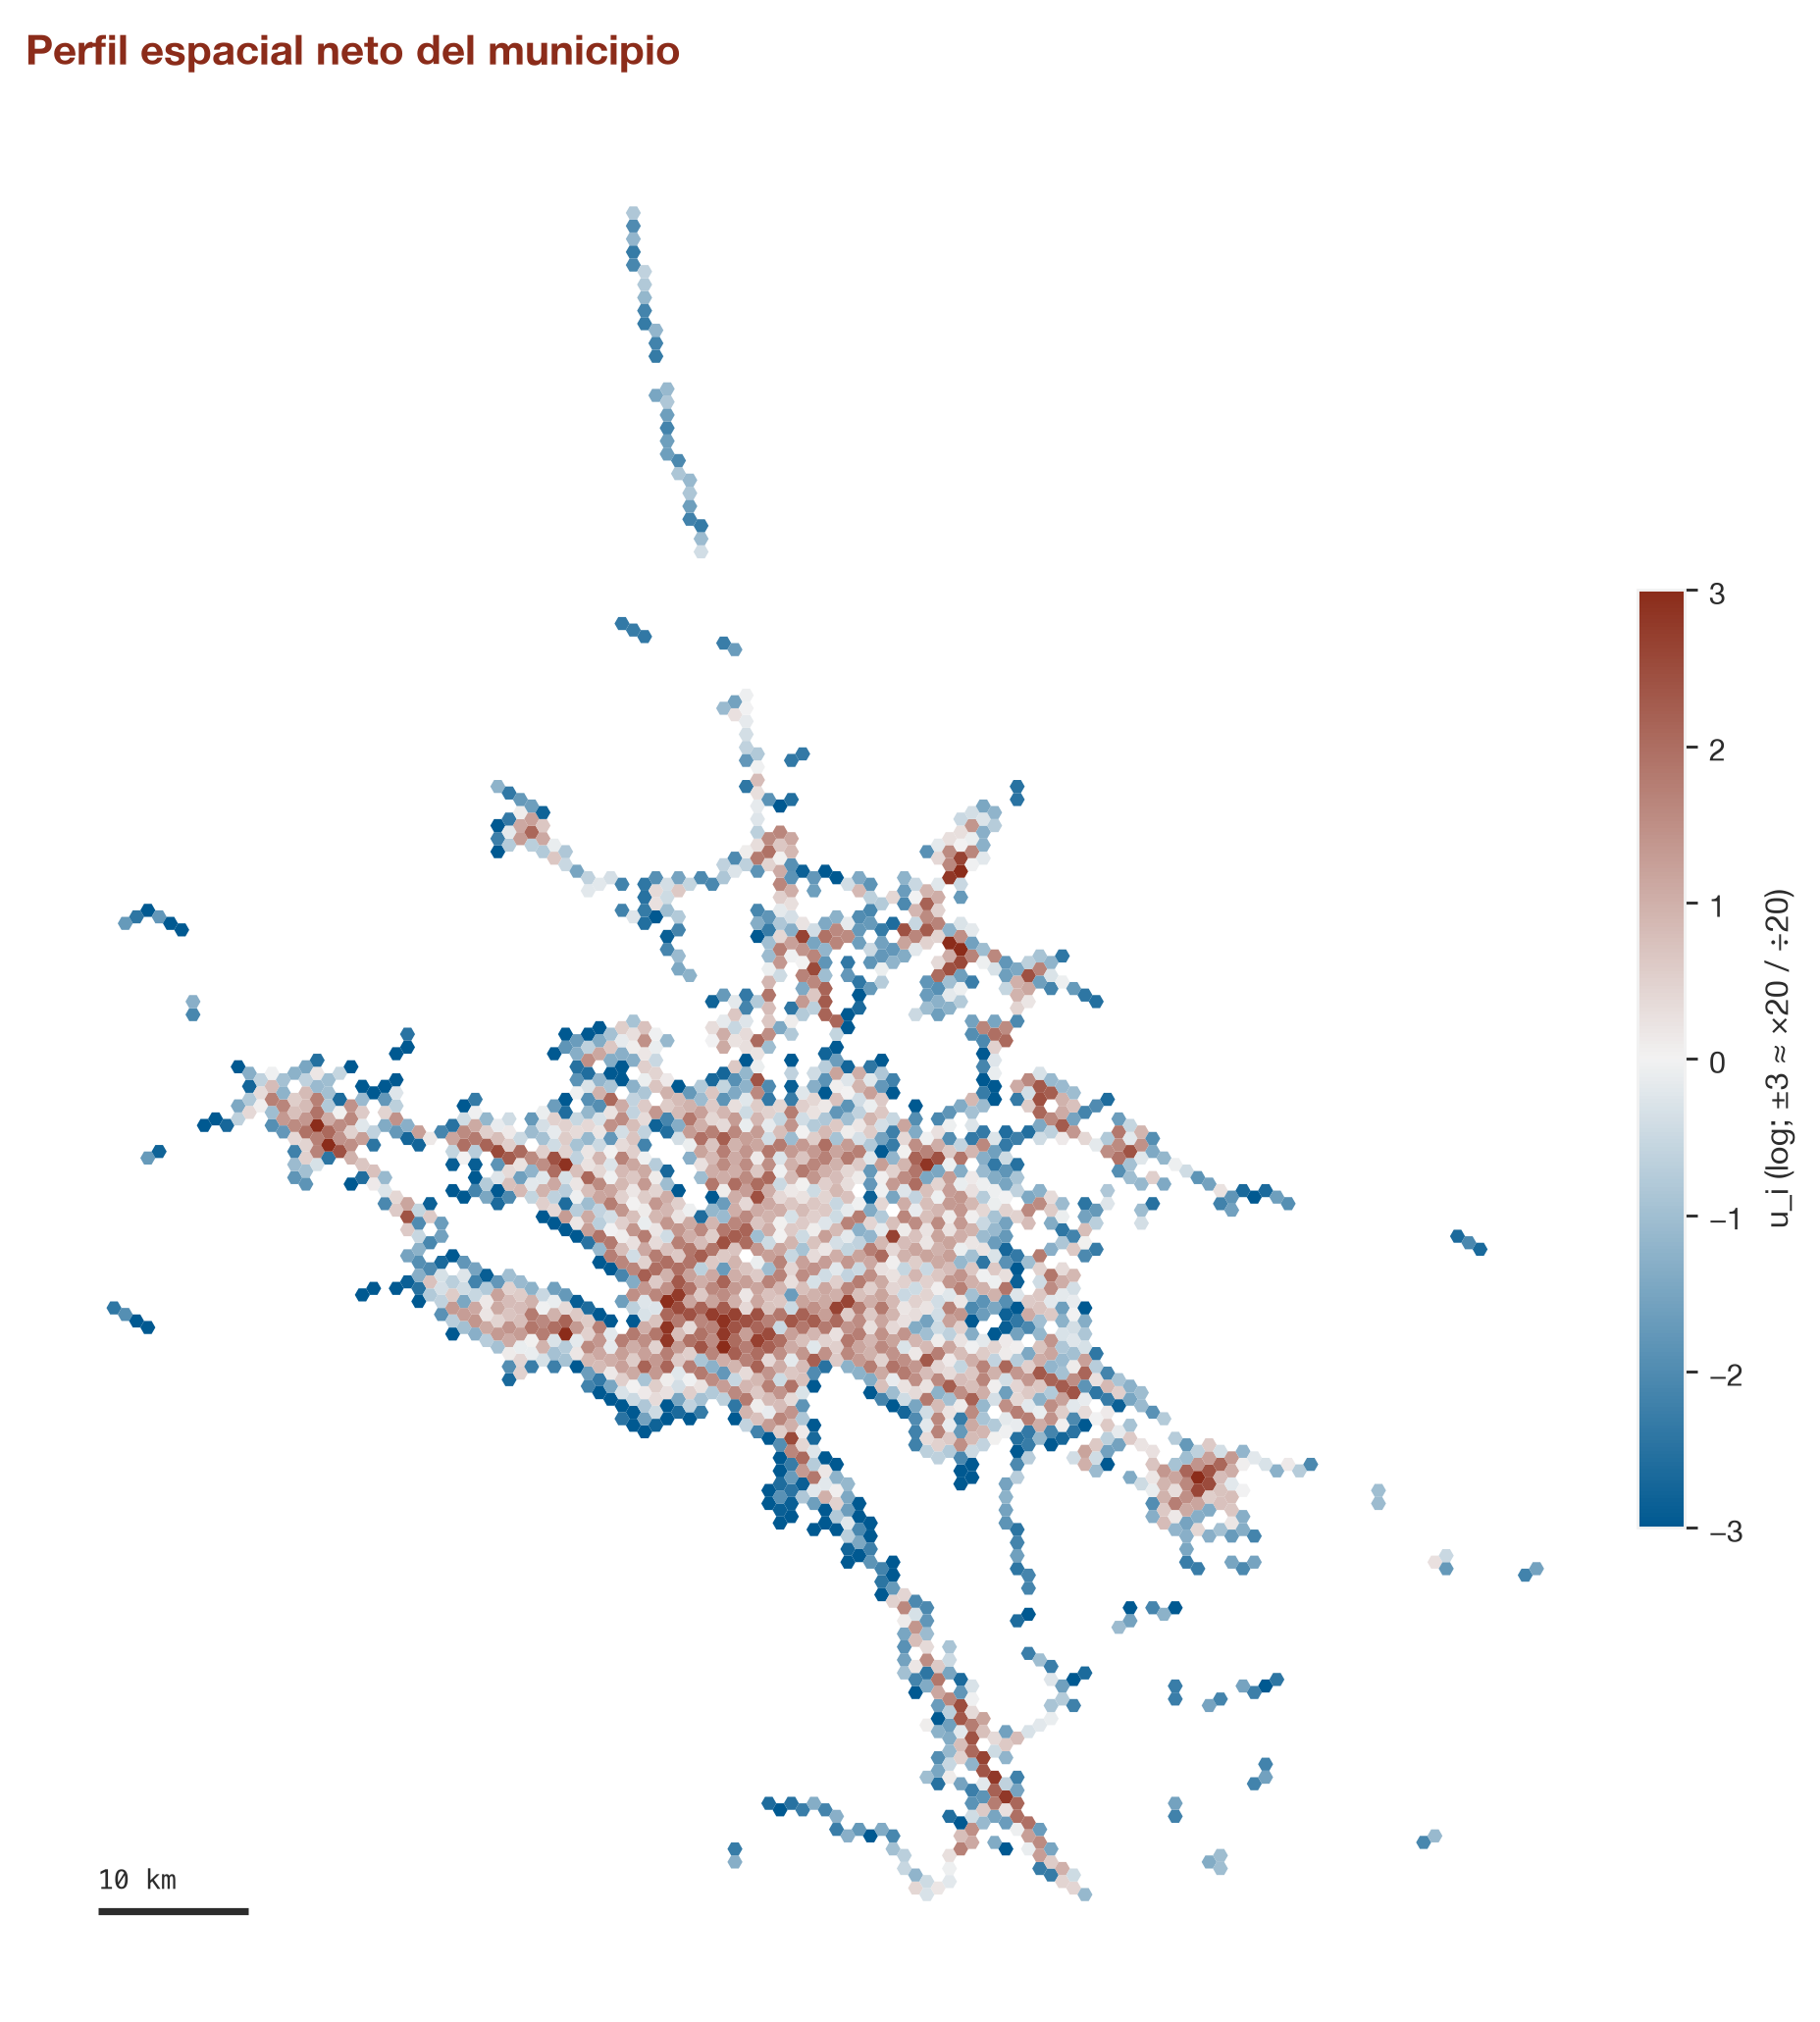
\includegraphics[width=0.80\textwidth]{perfil_u}
\caption{$u_i$: riesgo relativo de cada celda respecto a su municipio. Es el
primer mapa de la serie que no depende de cuánto reporta cada municipio:
Guadalupe se compara con Guadalupe. Los corredores aparecen en rojo; las
colonias interiores y los bordes, en azul.}
\end{figure}

\subsection{Validación en 2024}

El pronóstico es una simulación del modelo: para cada muestra posterior se
toma el nivel municipal de 2023, se combina con $u_i$ y se simula un conteo
Binomial Negativo. Los \emph{baselines} se recalculan a escala anual.

\begin{table}[H]
\centering\small
\begin{tabular}{lrrrr}
\toprule
Modelo (hex$\times$año) & MAE & CRPS & Cobertura 90\,\% & PAI 5\,\% \\
\midrule
M0 media 2019--23          & 9,59 & 8,04 & 63\,\% & 8,41 \\
M0r media 2022--23         & 8,15 & 6,56 & 68\,\% & 8,38 \\
M4 NB2, historia reciente  & 8,18 & 6,93 & 90\,\% & 8,38 \\
\textbf{M6 jerárquico CAR + municipio} & 8,19 & \textbf{6,17} & \textbf{87\,\%} & 8,42 \\
\bottomrule
\end{tabular}
\caption{Validación en 2024 a escala anual. El jerárquico calibra el total al
1\,\% (70\,815 predichos contra 71\,249 observados).}
\end{table}

El jerárquico \textbf{empata con M0r en MAE y lo supera en CRPS} (un 6\,\%). El
empate en MAE dice que la mediana de ambos apunta al mismo sitio: lo
predecible de 2024 es ``el nivel reciente de cada municipio por el perfil
estable de cada celda'', y un promedio bien elegido ya lo captura. La ventaja
en CRPS dice que la \emph{distribución} es mejor: el intervalo del 90\,\% de M0r
cubre el 68\,\% (es un Poisson que ignora la sobredispersión y el régimen); el
del jerárquico cubre el 87\,\%, sin incluir siquiera el riesgo de cambio de
régimen. Un intervalo que no cubre lo que dice cubrir no sirve para decidir.

\begin{advertencia}
\textbf{Por qué el pronóstico es por persistencia.} Pronosticar 2024 con una
innovación $t_3$ más es lo que el modelo sugiere, pero $\E[e^{T}] = \infty$
para cualquier $t$ de Student: ni la media predictiva ni el CRPS existen. Se
verificó numéricamente: la suma de medias con innovación $t$ dio 2,3 millones
contra 71 mil observados, y cambia con la semilla. El pronóstico es por tanto
\emph{condicional a que ningún municipio cambie de régimen en 2024}, y sus
intervalos son un piso de la incertidumbre real.
\end{advertencia}

Se probó además una \textbf{deriva por municipio} (tendencia local) para
capturar el crecimiento periférico: el modelo la encogió a cero
($\sigma_d = 0{,}07$), introdujo 46 divergencias y no mejoró el CRPS. Con cinco
años y saltos de régimen, los datos no distinguen una tendencia de una racha
de innovaciones. Se descartó.

% ===========================================================================
\section{Hallazgos transversales}
% ===========================================================================

\subsection{El PAI no se movió en ningún notebook}

Desde el análisis espacial hasta el jerárquico, el PAI al 5\,\% es 8,4. Es la
conclusión más firme del proyecto: \emph{el dónde lo decide el historial}, y
ningún término temporal ni espacial lo cambia. El \emph{shrinkage} reordena la
cola de la distribución, no la cabeza, que es donde se decide. Para mover el
PAI hacen falta covariables que varíen por celda y que el historial no
contenga —exposición vial, uso de suelo, población— y eso es dato externo.

\subsection{Lo que la base puede y no puede decir}

\begin{itemize}[leftmargin=1.4em]
\item Puede decir dónde se concentra el reporte de accidentes, con qué
  estructura espacial y con qué persistencia. Eso es robusto a todo lo que se
  probó.
\item Puede separar el nivel de reporte de cada municipio del perfil de cada
  celda, y estimar el segundo con la incertidumbre que corresponde.
\item No puede distinguir un municipio donde bajó el riesgo de uno que dejó
  de capturar accidentes. $m_{j,a}$ es reporte, no siniestralidad. Quien use
  los resultados debe hacer esa distinción por fuera.
\item No puede anticipar un cambio de régimen: que Santa Catarina empezara a
  reportar en 2022 o Guadalupe dejara de hacerlo en 2023 no está en los datos
  previos. Ese es el techo de medir siniestralidad con reportes
  administrativos, y hay que decirlo en cada entrega.
\end{itemize}

\subsection{Decisiones metodológicas que conviene recordar}

\begin{table}[H]
\centering\small
\begin{tabular}{p{4.2cm}p{9.6cm}}
\toprule
Decisión & Razón \\
\midrule
Hexágonos, no AGEB & Fronteras de AGEB sobre avenidas; área constante; vecindad regular \\
$\log(1+n)$ para Moran & La cola pesada dominaría un estadístico de productos cruzados; verificado con el crudo \\
FDR en todo mapa local & 2\,241 pruebas $\Rightarrow$ $\sim$112 falsos positivos; la corrección retira más de la mitad \\
NB2, no Poisson & Cameron--Trivedi $t=59$; rootograma \\
Sin ZINB & Los ceros en exceso son municipios sin reportar, no un segundo proceso \\
Sin $K$ de Ripley plana & Los eventos viven en la red; el nulo plano es imposible \\
Panel anual en el jerárquico & Separabilidad (M4 $\approx$ M0r) y cómputo \\
CAR propio, no BYM2 & BYM2 no se identifica con datos fuertes; documentado con los dos intentos \\
Innovaciones $t_3$ & Los saltos municipales inflaban $\sigma_{rw}$ al doble con normales \\
Pronóstico por persistencia & $\E[e^{T}]=\infty$; la media y el CRPS no existirían \\
Sin deriva municipal & Se encoge a cero, 46 divergencias, no mejora \\
Validación solo en 2024 & Un jerárquico con 2\,241 efectos ajusta el pasado casi perfecto; eso no es evidencia \\
\bottomrule
\end{tabular}
\end{table}

% ===========================================================================
\section{Siguientes pasos}
% ===========================================================================

En orden de costo--beneficio:

\begin{enumerate}[leftmargin=1.4em]
\item \textbf{Kilómetros de vialidad por celda} (OpenStreetMap o Red Nacional
  de Caminos). Es el mejor proxy de exposición disponible, entra como
  \emph{offset}, y es la única vía identificada para mover el PAI. Convierte el
  modelo de ``dónde hay accidentes'' en ``dónde hay más de los que el tráfico
  justifica''.
\item \textbf{Marco geoestadístico y Censo 2020} por AGEB, interpolados a
  hexágonos: población, densidad, marginación. Covariables de contexto.
\item \textbf{Modelo de severidad}, condicionado a que hubo accidente. Las
  variables consecuentes (tipo, vehículos, víctimas) son sus predictores
  naturales, y \texttt{TIPACCID}$\leftrightarrow$\texttt{gravedad} tiene la V de
  Cramér más alta de la base (0,49).
\item \textbf{Desagregación mensual} del pronóstico anual con el perfil
  estacional fijo, si hace falta operativamente.
\item Solo con la red vial ya descargada: $K$ de Ripley y KDE restringidas a
  red, como complemento descriptivo.
\end{enumerate}

% ===========================================================================
\appendix
\section{Reproducibilidad}
% ===========================================================================

Todo el pipeline está en el repositorio, en Python 3.14 gestionado con
\texttt{uv}. Los datos crudos (\texttt{data/raw/}) son las descargas del INEGI
sin modificar; todo lo demás se regenera:

\begin{verbatim}
uv sync
uv run consolidar-atus --geo     # raw -> parquet nacional
uv run zona-atus --geo           # recorte a la ZMM
uv run limpiar-atus --geo        # columnas derivadas (nunca borra ni imputa)
\end{verbatim}

Los notebooks son Quarto (\texttt{.qmd}) y cada uno tiene su PDF en
\texttt{docs/}: \texttt{calidad\_datos}, \texttt{analisis\_multivariado},
\texttt{analisis\_espacial}, \texttt{modelo\_conteo}, \texttt{modelo\_jerarquico}.
La partición hexagonal vive en \texttt{geostats.espacial} y los tres últimos
notebooks verifican que obtienen las mismas 2\,241 celdas.

\paragraph{Software.} \texttt{geopandas} 1.1, \texttt{libpysal}/\texttt{esda}
para pesos y estadísticos espaciales, \texttt{statsmodels} 0.15 para los GLM,
\texttt{PyMC} 6.3 con \texttt{nutpie} para el MCMC, \texttt{arviz} para
diagnósticos. Semilla 42 en todo; los resultados del MCMC se reproducen al
tercer decimal.

\section{Supuestos del modelo jerárquico y su verificación}

\begin{table}[H]
\centering\small
\begin{tabular}{p{4.4cm}p{6.2cm}p{2.6cm}}
\toprule
Supuesto & Verificación & Estado \\
\midrule
Separabilidad espacio-tiempo & Spearman 0,83 entre 2019 y 2024 & Apoyado \\
Régimen municipal como caminata aleatoria & Trayectorias a posteriori vs.\ series & Apoyado \\
Innovaciones de colas pesadas & $\sigma_{rw}$: 0,61 con normal, 0,29 con $t_3$ & Apoyado \\
Grafo de vecindad correcto y conexo & Sin islas; simetría verificada & Verificado \\
Convergencia del MCMC & $\Rhat$, ESS sobre $\log\mu$; 0 divergencias & Verificado \\
Priors no dictan el resultado & Reajuste con priors alternativos & Verificado \\
Subregistro estable por municipio & Series anuales por municipio & \textbf{Violado} \\
Sin cambio de régimen en 2024 & No verificable desde el pasado & Declarado \\
\bottomrule
\end{tabular}
\end{table}

\end{document}
